\documentclass[../../main.tex]{subfiles}

\begin{document}

\chapter{Quantum many-body framework}

This chapter is dedicated to introducing the necessary tools needed to perform realistic material calculations using dynamical mean-field theory (DMFT) or the dynamical vertex approximation $\dga$. We start with the most central objects - the Green's functions - and subsequently assemble a complete framework which enables us to calculate a number of physical properties, e.g. the susceptibility, optical conductivity, superconductivity, pseudogap formation and more, that stem from the correlated interplay between electrons or holes. 

\section{One-particle Green's functions}

Green's functions are fundamental tools in many-body physics, used to study the properties and behavior of interacting quantum systems. These mathematical objects encode information about the propagation of particles or excitations within a system and serve as the cornerstone for analyzing both equilibrium and nonequilibrium states. In the many-body regime, Green's functions extend beyond single-particle descriptions to include complex interactions among multiple particles. They provide insights into phenomena such as quasiparticle lifetimes, collective excitations and response functions. Specifically, one- and two-particle Green's functions describe the propagation of a single particle and the correlated motion of particle pairs, respectively. Alongside of the mathematical description of Green's function-based expressions, we also provide a pictorial description of the equations using Feynman diagrams. These Feynman diagrams allow us to easily describe interaction processes visually. Lines and vertices within the diagrams indicate particle propagators and interaction vertices, respectively. External legs will be colored gray while inner legs and interaction lines will be colored black.

In condensed matter physics, we are only interested in finite-temperature effects. Hence it is practical to use the so-called Matsubara formalism\cite{T. Matsubara. “A new approach to quantum-statistical mechanics”} in imaginary time by performing a Wick rotation $t\to -i\tau$\cite{G. C. Wick. “Properties of Bethe-Salpeter Wave Functions”}.

Furthermore, most many-body quantities described in the following are $n$-point (correlation) functions\footnote{Here, $n$ denotes the number of \say{connection points} of the corresponding Feynman diagram.}. These functions typically include a subset of the following parameters for each external leg: (Matsubara) frequency ($\nu$), spin index ($\sigma$), orbital index ($o$), lattice position ($\vv{R}$), momentum ($\vv{k}$) or imaginary time ($\tau$). This introduces a huge amount of parameters appended to a variable and can be very cumbersome to read through if explicitly written down. Therefore, to increase readability, we follow Ref.~\cite{N. E. Bickers and D. J. Scalapino. “Conserving approximations ...”} and group all indices that are not explicitly written down into a compound index, e.g. $\mathfrak{i}=\{o_i, \sigma_i, \vv{R}_i\}$. If an equation containing spatial or momentum-dependent quantities is written down with a compound index, it applies equally in both real and Fourier space. Furthermore, summing over these compound indices means summing over all individual components they include, with a normalization of $\frac 1\beta$ for frequency sums and $\frac{1}{N_{\vv{k}}}$ for momentum sums, where $\beta=\frac{1}{k_B T}$ is the inverse temperature and $N_{\vv{k}}$ is the total number of reciprocal lattice points. 
\\\\
After this short introduction, let us dive in by defining the most central quantity, the two-point (one-particle) Green's function, in a system in thermal equilibrium as
\begin{align}\label{eq:one_p_green_expectation_val}
	G_{\mathfrak{12}}^{\vv{k}}=-\mean{\mathcal{T}\left [\hat{c}_{\vv{k};\mathfrak{1}}\hat{c}^{\dagger}_{\vv{k};\mathfrak{2}}\right ]},
\end{align}
where $\hat{c}_{\vv{k};\mathfrak{i}}$ ($\hat{c}^{\dagger}_{\vv{k};\mathfrak{i}}$) are fermionic annihilation (creation) operators which annihilate (create) an electron with parameters $\mathfrak{i}=\{\sigma_i, o_i, \tau_i\}$ and momentum $\vv{k}$ in the system. $\mean{\cdot}=\frac{1}{Z}\trace{e^{-\beta\hat{\mathcal{H}}}\;\cdot }$ with $Z=\trace{e^{-\beta\hat{\mathcal{H}}}}$ describes the thermal expectation value. Note, that the time evolution operator $e^{i\hat{\mathcal{H}}t}=e^{\hat{\mathcal{H}}\tau}$ is real after performing the Wick rotation to imaginary time and the Boltzmann weight $e^{\beta\hat{\mathcal{H}}}$ describes nothing more than an additional evolution in imaginary time. Lastly, $\mathcal{T}[\cdot]$ is the imaginary time ordering operator, where
\begin{align}
	\mathcal{T}\left [\hat{c}^{(\dagger)}_{\mathfrak{1}}(\tau_1)\hat{c}^{(\dagger)}_{\mathfrak{2}}(\tau_2)\right ]=\Theta(\tau_1-\tau_2)\hat{c}^{(\dagger)}_{\mathfrak{1}}(\tau_1)\hat{c}^{(\dagger)}_{\mathfrak{2}}(\tau_2)-\Theta(\tau_2-\tau_1)\hat{c}^{(\dagger)}_{\mathfrak{2}}(\tau_2)\hat{c}^{(\dagger)}_{\mathfrak{1}}(\tau_1).
\end{align}
The Green's function measures the probability amplitude of a propagation process and reads as a Feynman diagram
\begin{figure}[ht!]
	\centering
	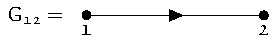
\includegraphics[scale=1.2]{../../Graphics/Diagrams/one_p_green/one_p_green}.
	\caption{Diagrammatic representation of the one-particle Green's function $G_{\mathfrak{12}}$. The electron is annihilated at $\mathfrak{1}$, propagates in imaginary time from $\tau_1$ to $\tau_2$ and is created at $\mathfrak{2}$.}
	\label{fig:one_p_green}
\end{figure}

In homogeneous systems, e.g., infinite or translationally invariant systems, the Green's function inherits the system's properties and becomes invariant under spatial translations. This means that $G_{\mathfrak{12}}(\vv{R}_1, \vv{R}_2)=G_{\mathfrak{12}}(\vv{R}_1-\vv{R}_2,\vv{0})=G_{\mathfrak{12}}(\vv{R})$. In Fourier space, this means that the Green's function is also only dependent on a single momentum parameter, $G_{\mathfrak{12}}(\vv{k}_1, \vv{k}_2)=G_{\mathfrak{12}}(\vv{k}_1-\vv{k}_2,\vv{0})=G_{\mathfrak{12}}(\vv{k})$. Furthermore, if the system is stationary, i.e., the Hamiltonian is not explicitly dependent on imaginary time, then $G_{\mathfrak{12}}(\tau_1, \tau_2)=G_{\mathfrak{12}}(\tau_1-\tau_2,0)=G_{\mathfrak{12}}(\tau)$. In absence of spin-orbit coupling, the spins at $\mathfrak{1}$ and $\mathfrak{2}$ need to be equal and therefore $G_{\mathfrak{12}}$ only depends on a single spin component. Additionally, the \textit{fermionic} Green's function can be shown to be anti-periodic in imaginary time with a period of $\beta$\footnote{This originates from the Boltzmann term $e^{\beta\hat{\mathcal{H}}}$ in the thermal expectation value and restricts the imaginary time domain to $\tau\in[-\beta,\beta)$.},
\begin{subequations}
\begin{align}
	G_{\mathfrak{12}}(\tau)&=-G_{\mathfrak{12}}(\beta-\tau)\quad\text{for } \tau>0 \qqand\\
	G_{\mathfrak{12}}(\tau)&=-G_{\mathfrak{12}}(\beta+\tau)\quad\text{for } \tau<0.
\end{align}
\end{subequations}
This anti-periodicity in time leads to the Fourier transform to be defined over a discrete set of imaginary frequencies, the the so-called Matsubara frequencies, which for fermionic quantities are given by $\nu_n=(2n+1)\frac\pi\beta$. In contrast, \textit{bosonic} Green's functions are periodic in imaginary time with period $\beta$ and therefore the Fourier transform includes the set of bosonic Matsubara frequencies $\omega_n=(2n)\frac\pi\beta$. In the following, we will always denote fermionic Matsubara frequencies with $\nu_n$ and bosonic ones with $\omega_n$. The fermionic- and bosonic-like Fourier transforms of $G_{\mathfrak{12}}(\tau)$ become, respectively,
\begin{align}
	G_{\mathfrak{12}}(i\nu_n)=\integral{0}{\beta}{\tau}G_{\mathfrak{12}}(\tau) e^{i\nu_n\tau} \qqand\qquad G_{\mathfrak{12}}(i\omega_n)=\integral{0}{\beta}{\tau}G_{\mathfrak{12}}(\tau) e^{i\omega_n\tau}
\end{align}
and only require the knowledge of Green's functions for positive imaginary times $\tau$. The inverse Fourier transforms are given by
\begin{align}
	G_{\mathfrak{12}}(\tau)=\frac1\beta \sum_n G_{\mathfrak{12}}(i\nu_n) e^{-i\nu_n\tau} \qqand\qquad G_{\mathfrak{12}}(\tau)=\frac1\beta \sum_n G_{\mathfrak{12}}(i\omega_n) e^{-i\omega_n\tau}.
\end{align}
If we perform a spectral representation of the fermionic Green's function in \eqref{eq:one_p_green_expectation_val} and calculate the discrete Fourier transform, we find that
\begin{align}
	G_{\mathfrak{12}}(i\nu_n)=\frac1Z\sum_{mn}\left (e^{-\beta E_n}+e^{-\beta E_m}\right )\frac{\sandwich{n}{\hat c_{\mathfrak{1}}}{m}\sandwich{m}{\hat c^{\dagger}_{\mathfrak{2}}}{n}}{i\nu-(E_m-E_n)}.
\end{align}
If we take $\mathfrak{1}\equiv \mathfrak{2}$, which corresponds to the \textit{local} Green's function, we can introduce the spectral function
\begin{align}
	A_{\mathfrak{1}}(\nu)=\frac1Z\sum_{mn} e^{-\beta E_n}\left (1+e^{-\beta\nu}\right ) |\sandwich{n}{\hat c_{\mathfrak{1}}}{m}|^2 \delta(\nu-E_m-E_n),
\end{align}
where
\begin{align}
	G_{\mathfrak{1}}(i\nu_n)=\integral{\mathbb{R}}{}{\nu}\frac{A_{\mathfrak{1}}(\nu)}{i\nu_n-\nu}.
\end{align}
The spectral function $A_{\mathfrak{1}}(\nu)$ is the probability of adding or removing a particle with momentum $\vv{k}_1$ with spin $\sigma_1$ from the system. For that reason, $A_{\mathfrak{1}}(\nu)$ is coined the single-particle local density of states. Furthermore, since it represents a probability distribution, the integral over all energies of $A_{\mathfrak{1}}(\nu)$ is equal to $1$. It is directly measurable using techniques like angle-resolved photoemission spectroscopy (ARPES) \cite{Quasiparticle spectral function, full momentum and energy resolved}, which probes electronic states in the material and reveals electronic structure properties, such as band gaps and quasiparticle dispersions. The peaks in $A_{\mathfrak{1}}(\nu)$ correspond to quasiparticle states, with their position indicating the energy of these states and their width related to the lifetime or decay rate of the quasiparticles. A narrow peak indicates a well-defined quasiparticle with a long lifetime and weak decay rate, while a broad peak suggests the contrary. The spectral function is a key quantity in many-body theory as it connects real-world experimental results to the Green's function formalism, as is shown in Refs. \cite{Quasiparticle spectral function, full momentum and energy resolved} and the following. By performing analytic continuation in the upper complex plane ($i\nu\to\nu+i0^{+}$), one can define the retarded Green's function as
\begin{align}
	G_{\mathfrak{1}}^{R}(\nu)=\integral{\mathbb{R}}{}{\nu'}\frac{A_{\mathfrak{1}}(\nu')}{\nu-\nu'+i 0^{+}},
\end{align}
from where one obtains through the Kramers-Kronig relations
\begin{align}
	A_{\mathfrak{1}}(\nu) = -\frac1\pi \Im G_{\mathfrak{1}}^{R}(\nu).
\end{align}
Thus, the spectral function is directly coupled to the imaginary part of the retarded Green's function, connecting many-body theory with physical experiments.

As an example, which will prove itself useful for the future, let us consider non-interacting electrons in a system with translational symmetry that are described by the (Wannier-) Hamiltonian
\begin{align}
	\hat{\mathcal{H}}_0=\sum_{\vv{k};\mathfrak{12}}\varepsilon_{\mathfrak{12}}(\vv{k})\hat c^{\dagger}_{\vv{k};\mathfrak{1}}\hat c_{\vv{k};\mathfrak{2}},
\end{align}
where $\varepsilon_{\mathfrak{12}}(\vv{k})=-\sum_{\vv{R};\mathfrak{12}} t_{\mathfrak{12}}(\vv{R})e^{i\vv{kR}}$ is the momentum dispersion of the band and is measured with respect to the chemical potential $\mu$. In this case, it is easy to show, that 
\begin{align}\label{eq:non_interacting_one_p_green}
	G_{0;\mathfrak{12}}(\nu, \vv{k})=[i\nu\delta_{\mathfrak{12}}-\varepsilon_{\mathfrak{12}}(\vv{k})]^{-1}.
\end{align}
For the one-particle spectral function, we find in this case 
\begin{align}
	A_{\mathfrak{12}}(\varepsilon,\vv{k})=\delta(\varepsilon-\varepsilon_{\vv{k};\mathfrak{12}}),
\end{align}
corresponding to stable quasiparticles, due to zero width of the quasiparticle peak of $A_{\mathfrak{12}}(\varepsilon,\vv{k})$.

The direct computation of the Green's function as expressed in \eqref{eq:one_p_green_expectation_val} generally incurs an exponential increase in cost with lattice size for interacting models. As a result, it is common practice to begin with the noninteracting case and construct a perturbative expansion in terms of the interaction around it. In this context, we will start with the non-interacting case described above. This perturbation expansion will not be derived in detail in this thesis, as there are many wonderful resources that explain it very thoroughly \cite{Abrikosov, Nolting}, thus we will only sketch it here. In essence, the expansion is constructed using the so-called $S$-matrix and employs strategies such as the Wick contraction \cite{Wick, evaluation of collision matrix and Notes on wick's theorem} and the linked cluster theorem \cite{linked cluster chapter in book}. The expansion begins by identifying the most general interaction part of the Hamiltonian of \eqref{eq:general_hubbard_hamiltonian},
\begin{align}
	\hat{\mathcal{H}}_{\text{I}} = \frac12 \sum_{\mathfrak{1234}}U_{\mathfrak{1234}}\hat c^{\dagger}_{\mathfrak{1}}\hat c^{\dagger}_{\mathfrak{3}}\hat c_{\mathfrak{4}}\hat c_{\mathfrak{2}}.
\end{align}
The expansion of the Green's function then reads
\begin{align}
	G_{\mathfrak{12}}(\tau)=-\frac{1}{\mean{S(\beta)}_0}\sum_{n=0}^{\infty}\frac{(-1)^n}{n!}\integral{0}{\beta}{\tau_1}\cdots\integral{0}{\beta}{\tau_n}\mean{\mathcal{T}\left [\hat{c}_{\mathfrak{1}}\hat{c}^{\dagger}_{\mathfrak{2}}\hat{\mathcal{H}}_{\text{I}}(\tau_1)\cdots \hat{\mathcal{H}}_{\text{I}}(\tau_n) \right ]}_0,
\end{align}
where $S(\beta)$ is the abovementioned $S$-matrix and $\mean{\cdot}_0$ is the thermal expectation value in terms of the non-interacting Hamiltonian $\hat{\mathcal{H}}_0$. 
In Feynman diagram jargon, this contains all diagrams that are possible, also disconnected ones\footnote{Disconnected means, that the term includes a diagram that consists of two separate, disconnected diagrams.}. The linked cluster theorem allows us to get rid of those disconnected contributions by effectively canceling with the $\frac{1}{\mean{S(\beta)}_0}$ term in front. This results in
\begin{align}\label{eq:one_p_green_full_perturbation_exp}
	G_{\mathfrak{12}}(\tau)=-\sum_{n=0}^{\infty}\frac{(-1)^n}{n!}\integral{0}{\beta}{\tau_1}\cdots\integral{0}{\beta}{\tau_n}\mean{\mathcal{T}\left [\hat{c}_{\mathfrak{1}}\hat{c}^{\dagger}_{\mathfrak{2}}\hat{\mathcal{H}}_{\text{I}}(\tau_1)\cdots \hat{\mathcal{H}}_{\text{I}}(\tau_n) \right ]}_0^{\text{conn}},
\end{align}
where $\mean{\cdot}_0^{\text{conn}}$ now indicates that we only consider connected diagrams in the expansion. We can transform this into a diagrammatic representation by applying Wick contractions, which allow us to collect pairs of creation and annihilation operators to form independent expectation values. In the case of the $n=1$ term in the perturbation expansion of the Green's function,
\begin{align}
\begin{split}
	G_{1;\mathfrak{12}}(\tau)=\sum_{\mathfrak{abcd}}&\integral{0}{\beta}{\tau_1}U_{\mathfrak{abcd}}\times\\
	&\times\bigg[- \mean{\mathcal{T}\left [\hat{c}_{\mathfrak{1}}(\tau)\hat{c}^{\dagger}_{\mathfrak{a}}(\tau_1)\right ]}_0 \mean{\mathcal{T}\left [\hat{c}_{\mathfrak{d}}(\tau_1)\hat{c}^{\dagger}_{\mathfrak{c}}(\tau_1)\right ]}_0 \mean{\mathcal{T}\left [\hat{c}_{\mathfrak{b}}(\tau_1)\hat{c}^{\dagger}_{\mathfrak{2}}(0)\right ]}_0\\
	&\qquad\!\!+\mean{\mathcal{T}\left [\hat{c}_{\mathfrak{1}}(\tau)\hat{c}^{\dagger}_{\mathfrak{a}}(\tau_1)\right ]}_0 \mean{\mathcal{T}\left [\hat{c}_{\mathfrak{b}}(\tau_1)\hat{c}^{\dagger}_{\mathfrak{c}}(\tau_1)\right ]}_0 \mean{\mathcal{T}\left [\hat{c}_{\mathfrak{d}}(\tau_1)\hat{c}^{\dagger}_{\mathfrak{2}}(0)\right ]}_0\bigg].
\end{split}
\end{align}
The remaining expectation values are nothing more than minus the non-interacting Green's function of \eqref{eq:non_interacting_one_p_green}. Written in Feynman diagrams, the first relevant perturbation expansion term is shown in \figref{fig:one_p_green_first_perturbation_term}.
\begin{figure}[ht!]
	\centering
	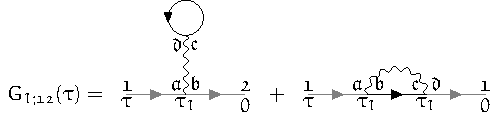
\includegraphics[scale=1.2]{../../Graphics/Diagrams/one_p_green_first_perturbation_term/one_p_green_first_perturbation_term}
	\caption{First order diagrams for the single-particle Green's function. The corresponding diagrams are coined the Hartree- and the Fock-term, respectively. As the name suggests, taking only these two diagrams as the whole perturbation expansion leads to the Hartree-Fock approximation, formulated as a diagrammatic theory.}
	\label{fig:one_p_green_first_perturbation_term}
\end{figure}

\section{Self-energy}

The one-particle Green's function perturbative expansion is already much simplified in the graphical portrayal. However, the number of diagrams increases exponentially with order $n$\footnote{For $n=2$ there exist $10$ diagrams, for $n=7$ the number of diagrams is well over a million.}. Therefore, the Feynman diagram approach would be of little practical use if the only way to progress was to calculate each diagram one at a time. However, in reality the technique is actually quite useful, since it hints on how to sum up the perturbative series. Let us talk about how it applies to Green's function for single particles. First, let us define another compound index which will further levitate readability. We will set $\k=\{\nu,\vv{k}\}$ and $\q=\{\omega, \vv{q}\}$ as a compound index including momentum and frequency in one index for fermionic ($\k$) and bosonic ($\q$) frequencies and momenta. Note, that if we write $\nu$ instead of $\k$, we refer to the \textit{local} part of the quantity with no momentum dependence instead of the \textit{non-local} part.

Diagrams in general can be split up into two classes: (i) diagrams that, by cutting a single internal Green's function line, transform in two lower-order diagrams, which are called one-particle reducible and (ii) diagrams that are not one-particle reducible, which are called one-particle irreducible (1PI). Let us define as the one-particle self-energy $\Sigma_{\mathfrak{12}}^{\k}$ the sum of all irreducible diagrams without external legs. For example, the black part of the diagrams in \figref{fig:one_p_green_first_perturbation_term} corresponds to the first-order diagrams of the self-energy. It is then straightforward to rewrite \eqref{eq:one_p_green_full_perturbation_exp} in terms of the self-energy, yielding
\begin{align}\label{eq:dyson_eq}
	G_{\mathfrak{12}}^{\k}=G_{0,\mathfrak{12}}^{\k}+\sum_{\mathfrak{ab}}G_{0,\mathfrak{1a}}^{\k}\Sigma_{\mathfrak{ab}}^{\k}G_{\mathfrak{b2}}^{\k},
\end{align}
which results in - when taking \eqref{eq:non_interacting_one_p_green} as the noninteracting Green's function and inverting in frequency and momentum space - a way to express the full (interacting) single-particle Green's function in terms of the self-energy
\begin{align}
	G_{\mathfrak{12}}^{\k} = \left [i\nu_n\delta_{\mathfrak{12}}-\varepsilon_{\mathfrak{12}}(\vv{k})-\Sigma_{\mathfrak{12}}^{\k}\right ]^{-1}.
\end{align}
\eqref{eq:dyson_eq} is commonly known as the Dyson equation \cite{dyson eq} for the single-particle Green's function and for completeness, its diagrammatic representation can be found in \figref{fig:dyson_eq}. It is a geometric series, where each term in the sum subsequently adds irreducible diagrams that are pieced together by non-interacting Green's functions to generate all possible diagrams.
\begin{figure}[ht!]
	\centering
	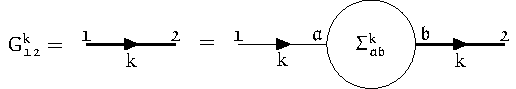
\includegraphics[scale=1.2]{../../Graphics/Diagrams/dyson_eq/dyson_eq}
	\caption{Diagrammatic representation of \eqref{eq:dyson_eq}. The full Green's function $G_{\mathfrak{12}}^{\k}$ is drawn as a thick black line.}
	\label{fig:dyson_eq}
\end{figure}
The self-energy can be obtained by simply inverting \eqref{eq:dyson_eq},
\begin{align}
	\Sigma_{\mathfrak{12}}^{\k}=(G_{0;\mathfrak{12}}^{\k})^{-1}-(G_{\mathfrak{12}}^{\k})^{-1}.
\end{align}
Thus, perturbation theory can be done in two distinct ways: the simpler approach is to determine the Green's function directly, for example, up to order $n$, where the second method is to compute the self-energy up to order $n$ and insert its expression in the Dyson equation \eqref{eq:dyson_eq}. This gives an approximate Green's function containing each order of perturbation theory with only a subset of all possible diagrams. As a result, \eqref{eq:dyson_eq} represents a way to sum up perturbation theory and is actually more relevant from a physical standpoint. Indeed, many methods leverage the usefulness of this approach, for example the dynamical mean-field theory or the dynamical vertex approximation, as we will see later.

Let us add some physical background to the self-energy in the following. $\Sigma$ represents the effects of the interaction on the single electron propagators. The real and imaginary part of the self-energy have significant impact on the physical properties of the system. The real part of the self-energy contributes to an energy shift of the electronic states of the single-particle energy levels $\varepsilon(\vv{k})$ due to interactions. In contrast, the imaginary part of the self-energy is related to the decay or lifetime of quasiparticles and introduces a spectral broadening or damping of the electronic states, indicating how long an excitation or quasiparticle persists before interacting with other excitations or scattering events. A larger imaginary part implies a shorter lifetime and stronger interactions. The first order derivative in frequency, $\dpd{\Sigma^{\k}}{\nu}$, contributes to an effective renormalization of the bare electron mass. It also leads to a redistribution of spectral weight in the one-particle spectral function, which provides information about the distribution of energy levels available for excitations. A broader spectral function, whose broadening is controlled by the imaginary part of the self-energy, typically indicates stronger interactions and a more correlated system.

\section{Two-particle Green's functions}

In analogy to the one-particle Green's function, the two-particle Green's function describes the amplitude of the propagation of two particles, two holes or a particle and a hole. A similar expression to \eqref{fig:one_p_green} can be formulated for the two-particle Green's function
\begin{align}
	G_{\mathfrak{1234}}^{\q\k\kp}=-\mean{\mathcal{T}\left [\hat{c}_{\vv{k};\mathfrak{1}}\hat{c}^{\dagger}_{\vv{k}-\vv{q};\mathfrak{2}}\hat{c}_{\vv{k}'-\vv{q};\mathfrak{3}}\hat{c}^{\dagger}_{\vv{k}';\mathfrak{4}}\right ]}.
\end{align}
It describes two particles, two holes or a particle and a hole being inserted in the system at times $\tau_2$ and $\tau_4$, propagating in the system until they are removed again at $\tau_1$ and $\tau_3$, respectively. Assuming a stationary Hamiltonian that satisfies time-translation invariance, it is possible to eliminate one imaginary time variable by setting it zero. Then, the Green's function only depends on three time variables and through Fourier transform, also only depends on three frequency and momentum variables. 
Furthermore, similar to the case for the one-particle Green's function, the absence of spin-orbit coupling reduces the number of spin degrees of freedom 
\begin{subequations}
\begin{align}
	G_{\ss';\mathfrak{1234}}^{\q\k\kp}&=G_{\ss\sigma'\sigma';\mathfrak{1234}}^{\q\k\kp} \qqand\\
	G_{\overline{\ss'};\mathfrak{1234}}^{\q\k\kp}&=G_{\ss'\sigma'\sigma;\mathfrak{1234}}^{\q\k\kp}.
\end{align}
\end{subequations}
In this case, the total incoming and outgoing spin must be equal and this puts a heavy constraint on the possible spin combinations,
\begin{align}
	\sigma_1=\sigma_2=\sigma_3=\sigma_4, \qquad (\sigma_1=\sigma_2) \neq (\sigma_3=\sigma_4)\qqand\qquad (\sigma_1=\sigma_4)\neq(\sigma_2=\sigma_3),
\end{align}
totaling to only six unique spin combinations, each of which can be seen in \figref{fig:two_particle_green_spins}.
\begin{figure}[h]
  \centering
  \subfloat{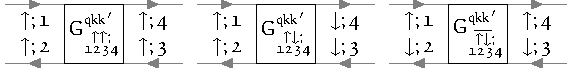
\includegraphics[scale=1.2]{../../Graphics/Diagrams/two_particle_green_spins/two_particle_green_spins_row1}}\vspace{0.5cm}\\
  \subfloat{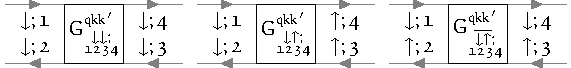
\includegraphics[scale=1.2]{../../Graphics/Diagrams/two_particle_green_spins/two_particle_green_spins_row2}}
  \caption{In the case of absent spin-orbit coupling, these are the only non-vanishing spin combinations of the two-particle Green's function.}
  \label{fig:two_particle_green_spins}
\end{figure}
Furthermore, if one describes quantities in the paramagnetic phase, where the system is SU(2)-symmetric, there are only two independent spin configurations,
\begin{subequations}
\begin{align}
	G_{\ss';\mathfrak{1234}}^{\q\k\kp}&=G_{(-\sigma)(-\sigma');\mathfrak{1234}}^{\q\k\kp}=G_{\sigma'\sigma;\mathfrak{1234}}^{\q\k\kp}\qqand\\
	G_{\ss;\mathfrak{1234}}^{\q\k\kp}&=G_{\sigma(-\sigma);\mathfrak{1234}}^{\q\k\kp}+G_{\overline{\sigma(-\sigma)};\mathfrak{1234}}^{\q\k\kp}.
\end{align}
\end{subequations}
For these two spin combinations, the (d)ensity, (m)agnetic, (s)inglet and (t)riplet channel\footnote{As we will see later, in $\ph/\phbar$-notation, the Bethe-Salpeter equation will become diagonal for the $\dens/\magn$ spin combination as well as for pp-notation in the $\sing/\trip$ spin combination.} specified in the following are a particularly helpful choice of notation, as we shall see in the upcoming sections: 
\begin{subequations}
\begin{align}
	G_{\dens;\mathfrak{1234}}^{\q\k\kp}&=G_{\uparrow\uparrow;\mathfrak{1234}}^{\q\k\kp}+G_{\uparrow\downarrow;\mathfrak{1234}}^{\q\k\kp},\label{eq:two_particle_green_density}\\
	G_{\magn;\mathfrak{1234}}^{\q\k\kp}&=G_{\uparrow\uparrow;\mathfrak{1234}}^{\q\k\kp}-G_{\uparrow\downarrow;\mathfrak{1234}}^{\q\k\kp}=G_{\overline{\uparrow\downarrow};\mathfrak{1234}}^{\q\k\kp},\label{eq:two_particle_green_magnetic}\\
	G_{\sing;\mathfrak{1234}}^{\q\k\kp}&=G^{\q\k\kp}_{\uparrow\downarrow;\mathfrak{1234}}-G^{\q\k\kp}_{\overline{\uparrow\downarrow};\mathfrak{1234}}\qqand\\
	G_{\trip;\mathfrak{1234}}^{\q\k\kp}&=G^{\q\k\kp}_{\uparrow\downarrow;\mathfrak{1234}}+G^{\q\k\kp}_{\overline{\uparrow\downarrow};\mathfrak{1234}}.
\end{align}
\end{subequations}
Besides the spin-symmetries discussed above, the Green's function also inherits other properties of the system, such as time-reversal symmetry, which manifests itself by
\begin{align}
	G_{\mathfrak{1234}}^{\q\k\kp}=G_{\mathfrak{4321}}^{\bar\q\bar{\k}'\bar\k},
\end{align} 
where $\overline\k=\{\nu,-\vv{k}\}$ is the time-reversed compound momentum variable. Furthermore, the two-particle Green's function satisfies the crossing symmetry, which is a direct manifestation of Pauli's principle. Crossing symmetry refers to the antisymmetric property of the Green's function with respect to the exchange of the incoming and outgoing fermions
\begin{subequations}
\begin{align}
	G_{\ss';\mathfrak{1234}}^{\q\k\kp}&= -G_{\overline{\sigma'\sigma};\mathfrak{3214}}^{(\kp-\k)(\kp-\q)\kp}\label{eq:crossing_sym_1}\\
	&= -G_{\overline{\ss'};\mathfrak{1432}}^{(\k-\kp)\k(\k-\q)}\label{eq:crossing_sym_2}\\
	&= G_{\sigma'\sigma;\mathfrak{3412}}^{(-\q)(\kp-\q)(\k-\q)}.\label{eq:crossing_sym_3}
\end{align}
\end{subequations}
The symmetries \eqref{eq:crossing_sym_1} - \eqref{eq:crossing_sym_3} describe the frequency changes that occur by exchanging the positions of the gray fermion lines, leaving the vertex unchanged. The last line corresponds to a full swap of the incoming and outgoing particle labels. The crossing symmetry is visually shown in \figref{fig:two_particle_green_crossing_symmetry}. Lastly, the Green's function also possesses symmetry with respect to complex conjugation,
\begin{align}
	\left (G_{\ss';\mathfrak{1234}}^{\q\k\kp}\right )^*=G_{\sigma'\sigma;\mathfrak{4321}}^{(-\q)(-\k)(-\kp)}.
\end{align}
\begin{figure}[h]
  \centering
  \subfloat{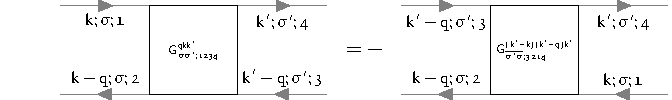
\includegraphics[scale=1.4]{../../Graphics/Diagrams/two_particle_green_crossing_symmetry/two_particle_green_crossing_symmetry_row1}}\vspace{0.5cm}\\
  \subfloat{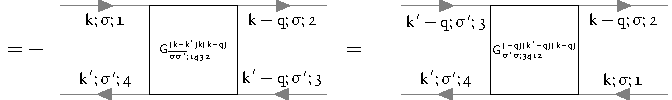
\includegraphics[scale=1.4]{../../Graphics/Diagrams/two_particle_green_crossing_symmetry/two_particle_green_crossing_symmetry_row2}}
  \caption{Diagrammatic representation of the crossing symmetry relations in order of \eqref{eq:crossing_sym_1} - \eqref{eq:crossing_sym_3}.}
  \label{fig:two_particle_green_crossing_symmetry}
\end{figure}
At the beginning of the section it was stated that the (four-point) two-particle Green's function only requires three frequency arguments to be fixed since the last one is automatically given by momentum conservation. There are three equivalent choices (coined channels) of independent frequencies (with $\nu$, $\nu'$ being a fermionic and $\omega$ a bosonic Matsubara frequency)
\begin{subequations}
\begin{align}
	\text{ph-notation:}&\;\;\{\nu_1=\nu,&&\nu_2=\nu-\omega,&&\nu_3=\nu'-\omega,&&\nu_4=\nu'\},\label{eq:ph_freq}\\
	\phbar\text{-notation:}&\;\;\{\nu_1=\nu,&&\nu_2=\nu',&&\nu_3=\nu'-\omega,&&\nu_4=\nu-\omega\}\qqand\label{eq:ph_bar_freq}\\
	\text{pp-notation:}&\;\;\{\nu_1=\nu,&&\nu_2=\omega-\nu',&&\nu_3=\omega-\nu,&&\nu_4=\nu'\}.\label{eq:pp_freq}
\end{align}
\end{subequations}
To show the effects of this frequency shift and how they affect the labels of the diagrams, we show the two-particle Green's function in the three notations of \eqref{eq:ph_freq} - \eqref{eq:pp_freq} in \figref{fig:two_particle_green_channels} below.
\begin{figure}[h]
  \centering
  \subfloat{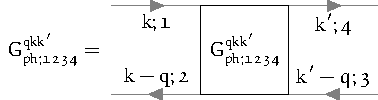
\includegraphics[scale=1.2]{../../Graphics/Diagrams/two_particle_green_channels/two_particle_green_channels_ph}}\vspace{0.5cm}\\
  \subfloat{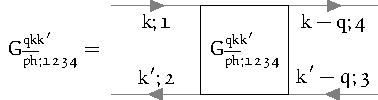
\includegraphics[scale=1.2]{../../Graphics/Diagrams/two_particle_green_channels/two_particle_green_channels_ph_bar}}\vspace{0.5cm}\\
  \subfloat{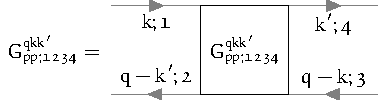
\includegraphics[scale=1.2]{../../Graphics/Diagrams/two_particle_green_channels/two_particle_green_channels_pp}}
  \caption{Two-particle Green's functions in the different frequency notations of \eqref{eq:ph_freq} - \eqref{eq:pp_freq} expressed in Feynman diagrams. The frequency notation is encoded in an additional subscript, $\{\ph, \phbar,\pp\}$.}
  \label{fig:two_particle_green_channels}
\end{figure}
Obviously, the choice of frequency convention should not have any impact on the physical content of the Green's function, hence it is possible to switch between these channels by applying channel-specific frequency shifts \cite{continuous qmc asympt},
\begin{subequations}
\begin{align}
	G_{\ph;\mathfrak{1234}}^{\q\k\kp}&=G_{\phbar;\mathfrak{1234}}^{(\k-\kp)\k(\k-\q)},\\
	G_{\phbar;\mathfrak{1234}}^{\q\k\kp}&=G_{\ph;\mathfrak{1234}}^{(\k-\kp)\k(\k-\q)},\\
	G_{\ph;\mathfrak{1234}}^{\q\k\kp}&=G_{\pp;\mathfrak{1234}}^{(\k+\kp-\q)\k\kp}\qqand\\
	G_{\pp;\mathfrak{1234}}^{\q\k\kp}&=G_{\ph;\mathfrak{1234}}^{(\k+\kp-\q)\k\kp}.
\end{align}
\end{subequations}
Let us finally note that the two-particle Green's function represents all diagrams that are possible that involve two electrons, two holes or an electron and a hole. It can therefore be split into two parts: (i) a part, where the electrons do not interact with each other and propagate independently; and (ii) a part, where the electrons do interact with each other through an infinite number of processes. (ii) is commonly called the connected two-particle Green's function and can be mathematically formulated by
\begin{align}\label{eq:two_particle_green_connected}
	G_{\ss';\mathfrak{1234}}^{\q\k\kp}=G_{\ss';\mathfrak{1234}}^{\text{conn};\q\k\kp}+\delta_{\q0}G_{\sigma;\mathfrak{12}}^{\k}G_{\sigma';\mathfrak{34}}^{\kp}-\delta_{\ss'}\delta_{\k\kp}G_{\sigma;\mathfrak{14}}^{\k}G_{\sigma;\mathfrak{32}}^{\k-\q}.
\end{align}
Diagrammatically, the connected two-particle Green's function contains all diagrams, where two propagating electrons interact with each other. The first terms up to interaction order two are given in \figref{fig:two_particle_green_connected}.
\begin{figure}[h]
  \centering
  \subfloat{\includestandalone[width=\textwidth]{../../Graphics/Diagrams/two_particle_green_connected/two_particle_green_connected_separate_row1}}\vspace{0.5cm}\\
  \subfloat{\includestandalone[width=\textwidth]{../../Graphics/Diagrams/two_particle_green_connected/two_particle_green_connected_separate_row2}}\vspace{0.5cm}\\
  \subfloat{\includestandalone[width=\textwidth]{../../Graphics/Diagrams/two_particle_green_connected/two_particle_green_connected_separate_row3}}
  \caption{Diagrammatic representation of the two-particle connected Green's function up to order two. It includes the possible interaction processes that occur between two propagating electrons. The particle labels are only written down for the first diagram, the other diagrams are labeled analogously.}
  \label{fig:two_particle_green_connected}
\end{figure}
The other terms in \eqref{eq:two_particle_green_connected} are not that interesting, they merely describe the electrons propagating in the system without ever interacting with the other. However, we will still show the diagrammatic content of the second and third term of \eqref{eq:two_particle_green_connected} in \figref{fig:two_particle_green_disconnected}.
\begin{figure}[ht!]
	\centering
	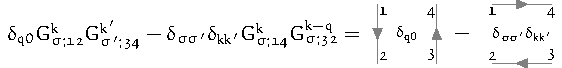
\includegraphics[scale=1.2]{../../Graphics/Diagrams/two_particle_green_disconnected/two_particle_green_disconnected}
	\caption{Disconnected part (second and third term on the right hand side of \eqref{eq:two_particle_green_connected}) of the two-particle Green's function.}
	\label{fig:two_particle_green_disconnected}
\end{figure}
The connected two-particle Green's function without the external legs is commonly called the full vertex $F$, where by convention an additional minus sign is introduced,
\begin{align}
	G_{\mathfrak{1234}}^{\text{conn};\q\k\kp} = -\frac1\beta \sum_{\mathfrak{abcd}} G_{\mathfrak{1a}}^{\k} G_{\mathfrak{b2}}^{\k-q} F_{\mathfrak{abcd}}^{\q\k\kp} G_{\mathfrak{3c}}^{\kp-q} G_{\mathfrak{d4}}^{\kp}.
\end{align}
By the previous definition, the vertex function $F_{\mathfrak{1234}}^{\q\k\kp}$ contains all diagrams that connect two incoming and two outgoing lines. All diagrams contained in the full vertex $F_{\mathfrak{1234}}^{\q\k\kp}$ can be classified by their two-particle reducibility (2PR). A diagram is called two-particle reducible, if it can be split into two separate parts by cutting two internal Green's function lines. Furthermore, this classification is described by three channels, $\{\ph,\phbar,\pp\}$\footnote{The attentive reader remembers that there are also three (identically-named) frequency notations that were mentioned previously. The channel reducibility and frequency notation are - in general - detached. From now on, if only one subscript $\r\in\{\ph,\phbar,\pp\}$ is given per vertex quantity, it means that the channel reducibility will belong to $\r$ and the frequency notation will be $\ph$-like. Otherwise, the channel reducibility and frequency notation will be denoted in the sub- and superscript of the variable separately. This will be relevant later when discussing the Bethe-Salpeter equation (BSE), see \secref{sec:bethe_salpeter}. The BSE is only diagonal in the bosonic transfer momentum and frequency $\q$ if the channel reducibility is the same as the frequency notation.}, depending on which incoming and outgoing lines are being separated by this \say{cutting}-process. The $\ph$-channel corresponds to those diagrams, where the sub-parts connect $\mathfrak{12}$ and $\mathfrak{34}$, for the $\phbar$-channel $\mathfrak{14}$ and $\mathfrak{23}$ and for the $\pp$-channel $\mathfrak{13}$ and $\mathfrak{24}$ are connected. These reducible diagrams are categorized in $\Phi_{\ph;\mathfrak{1234}}^{\q\k\kp}$, $\Phi_{\phbar;\mathfrak{1234}}^{\q\k\kp}$ and $\Phi_{\pp;\mathfrak{1234}}^{\q\k\kp}$, respectively. All diagrams that are not two-particle reducible are grouped together in the quantity $\Lambda_{\mathfrak{1234}}^{\q\k\kp}$. This procedure is called the parquet decomposition and reads mathematically
\begin{align}\label{eq:parquet_decomposition}
	F_{\mathfrak{1234}}^{\q\k\kp}=\Lambda_{\mathfrak{1234}}^{\q\k\kp}+\Phi_{\ph;\mathfrak{1234}}^{\q\k\kp}+\Phi_{\phbar;\mathfrak{1234}}^{\q\k\kp}+\Phi_{\pp;\mathfrak{1234}}^{\q\k\kp}.
\end{align}
Another possibility is to split up the full vertex $F$ in reducible and irreducible diagrams in a specific channel $\r\in\{\ph,\phbar,\pp\}$,
\begin{align}\label{eq:full_vertex_gamma_phi}
	F_{\mathfrak{1234}}^{\q\k\kp}=\Gamma_{\r;\mathfrak{1234}}^{\q\k\kp}+\Phi_{\r;\mathfrak{1234}}^{\q\k\kp},
\end{align}
where $\Gamma_{\r;\mathfrak{1234}}^{\q\k\kp}$ is the irreducible vertex in channel $\r$ and $\Phi_{\r;\mathfrak{1234}}^{\q\k\kp}$ the corresponding reducible one. Note, that in channel $\r$ irreducible diagrams might still be reducible in another channel $\r'\neq \r$. For example, $\Gamma_{\ph;\mathfrak{1234}}^{\q\k\kp}$ contains all fully irreducible diagrams, but also all diagrams which are reducible in channels $\phbar$ and $\pp$,
\begin{align}
	\Gamma_{\ph;\mathfrak{1234}}^{\q\k\kp}=\Lambda_{\mathfrak{1234}}^{\q\k\kp}+\Phi_{\phbar;\mathfrak{1234}}^{\q\k\kp}+\Phi_{\pp;\mathfrak{1234}}^{\q\k\kp}.
\end{align}
This will be important later in \secref{sec:bethe_salpeter}, where we will discuss the Bethe-Salpeter equations. Furthermore, the following relations for the ph and $\phbar$ channel for $\Gamma_{\r;\mathfrak{1234}}^{\q\k\kp}$ and $\Phi_{\r;\mathfrak{1234}}^{\q\k\kp}$ hold:
\begin{subequations}\label{eq:phi_conversion_ph_bar_to_ph}
\begin{align}
	\Phi_{\phbar;\mathfrak{1234};\ss'}^{\q\k\kp}&=-\Phi_{\ph;\mathfrak{3214};\overline{\sigma'\sigma}}^{(\kp-\k)(\kp-\q)\kp},\\
	&=-\Phi_{\ph;\mathfrak{1432};\overline{\sigma'\sigma}}^{(\k-\kp)\k(\k-\q)}.
\end{align}
\end{subequations}
From this one can construct the density and magnetic contributions to $\Phi_{\phbar;\mathfrak{1234};\ss'}^{\q\k\kp}$ in terms of $\Phi_{\ph;\mathfrak{1234};\ss'}^{\q\k\kp}$
\begin{subequations}\label{eq:phi_ph_bar_dens_magn}
\begin{align}
	\Phi_{\dens;\phbar;\mathfrak{1234}}^{\q\k\kp}&=-\frac12\Phi_{\dens;\ph;\mathfrak{3214}}^{(\kp-\k)(\kp-\q)\kp}-\frac32\Phi_{\magn;\ph;\mathfrak{3214}}^{(\kp-\k)(\kp-\q)\kp}\\
	\Phi_{\magn;\phbar;\mathfrak{1234}}^{\q\k\kp}&=-\frac12\Phi_{\dens;\ph;\mathfrak{3214}}^{(\kp-\k)(\kp-\q)\kp}+\frac12\Phi_{\magn;\ph;\mathfrak{3214}}^{(\kp-\k)(\kp-\q)\kp}.
\end{align}
\end{subequations}
The relations \eqref{eq:phi_conversion_ph_bar_to_ph} and \eqref{eq:phi_ph_bar_dens_magn} also apply to the full- and irreducible vertices $F_{\phbar;\mathfrak{1234};\ss'}^{\q\k\kp}$ and $\Gamma_{\phbar;\mathfrak{1234};\ss'}^{\q\k\kp}$ in a similar fashion. Note that there is no connection between the pp channel and the other two channels, hence it is not possible to transform the channel reducibility from either ph or $\phbar$ to pp. The pp-channel fulfills a crossing symmetry on its own,
\begin{align}
	\Phi^{\q\k\kp}_{\pp;\mathfrak{1234};\ss'}=-\Phi^{(\k-\kp)\k(\k-\q)}_{\pp;\mathfrak{1432};\overline{\ss'}}.
\end{align}

As the next step, let us briefly introduce the concept of linear response and the central physical property describing the response of a system with respect to an external perturbation\footnote{For example an external electromagnetic field.}, the susceptibility.

\section{Susceptibility}

Experimentally, it is not possible to directly extract information (just by \say{looking}) about the interactions between electrons in a system. Instead, in spectroscopic experiments, a perturbation is applied to the system and one measures the system's response. In particular, one measures how expectation values $\mean{\cdot}$ of operators (take the multi-dimensional operator $\hat O_{i}(\tau)$ as an example) changes when an external field $h_{j}(\tau)$ is applied. In linear response theory, this response is --- as the name suggests --- taken to be linear in the perturbing field, requiring this field to be sufficiently small in order for this description to be a good approximation \cite{kappl susc},
\begin{align}
	\mean{\hat O_{i}(\tau)}_{\vv{h}}-\mean{\hat O_{i}(\tau)}_{\vv{h}=0}=\integral{0}{\beta}{\tau'} \chi_{ij}(\tau-\tau')h_{j}(\tau')+\mathcal{O}(\vv{h}^2),
\end{align}
where $\chi_{ij}(\tau-\tau')$ is coined physical susceptibility and does not depend on the field $h_{j}(\tau)$. $\chi(\tau-\tau')$ fulfills the Kramers-Kronig relations, is causal ($\chi_{ij}(\tau-\tau')=\Theta(\tau-\tau')\chi_{ij}(\tau-\tau')$) and is finite ($\forall\, \tau,\tau':\;\exists\, C\in\mathbb{R}:\; |\chi_{ij}(\tau-\tau')|<C$). The susceptibility can be computed straightforwardly by taking the functional derivative of $\hat O_{i}(\tau)$ with respect to the field $h_{j}(\tau)$,
\begin{align}
	\chi_{ij}(\tau-\tau')=\ddd{\mean{\hat O_{i}(\tau')}}{h_{j}(\tau)}\bigg|_{\vv{h}=0}=\mean{\mathcal{T}\hat O_{i}(\tau)\hat O_{j}(\tau')}-\mean{\hat O_{i}}\mean{\hat O_{j}}.
\end{align}
On the two-particle level, only the density's response to variations in the one-particle energy, $\chi_{\dens}$, and the magnetization's response to variation in the electromagnetic field in the same direction, $\chi_{\magn}$, are non-zero \cite{kappl susc},
\begin{subequations}
\begin{alignat}{3}
	\chi_{\dens}(\tau)&=\chi_{nn}(\tau)&&=-&&\ddd{\mean{\hat n}}{\mu(\tau)}\bigg|_{\mu=0}\qqand\label{eq:chi_dens_derivative}\\
	\chi_{\magn}(\tau)&=\chi_{ii}(\tau)&&=&&\ddd{\mean{\hat\sigma_{i}}}{h_{i}(\tau)}\bigg|_{\vv{h}=0},\label{eq:chi_magn_derivative}
\end{alignat}
\end{subequations}
where $i\in\{x,y,z\}$. The physical susceptibilities are included in the two-particle Green's function, as we will see shortly. In fact, the sum of terms corresponding to the two disconnected, horizontal Green's function lines and the vertex part is denoted as the generalized susceptibility and can be expressed as
\begin{align*}\label{eq:generalized_susceptibility}
	\chi_{\mathfrak{1234}}^{\ph;\q\k\kp}&=\beta\left (G_{\mathfrak{1234}}^{\ph;\q\k\kp}-\delta_{q0}G_{\mathfrak{14}}^{\k} G_{\mathfrak{32}}^{\kp}\right )\\
	&=-\beta\delta_{\k\kp}G_{\mathfrak{14}}^{\k}G_{\mathfrak{32}}^{\k-\q}-\sum_{\mathfrak{abcd}} G_{\mathfrak{1a}}^{\k} G_{\mathfrak{b2}}^{\k-q} F_{\mathfrak{abcd}}^{\ph;\q\k\kp} G_{\mathfrak{3c}}^{\kp-q} G_{\mathfrak{d4}}^{\kp}\\
	&=\chi_{0;\mathfrak{1234}}^{\q\k\kp}-\frac{1}{\beta^2}\sum_{\mathfrak{abcd}}\chi_{0;\mathfrak{12ba}}^{\q\k\k} F_{\mathfrak{abcd}}^{\ph;\q\k\kp} \chi_{0;\mathfrak{dc34}}^{\q\kp\kp},\numberthis
\end{align*}
where
\begin{align}
	\chi_{0;\mathfrak{1234}}^{\q\k\kp}=-\beta\delta_{\k\kp}G_{\mathfrak{14}}^{\k}G_{\mathfrak{32}}^{\k-\q}
\end{align}
is commonly denoted as the generalized bubble susceptibility\footnote{The generalized susceptibility in the particle-particle channel reads
\begin{align}\label{eq:generalized_susceptibility_pp_ssp}
	\chi_{\mathfrak{1234};\ss'}^{\pp;\q\k\kp}=\beta\left (1-\delta_{\ss'}\right )\left [G_{\mathfrak{1234};\ss'}^{\pp;\q\k\kp}-\delta_{q0}G_{\mathfrak{14}}^{-\k} G_{\mathfrak{32}}^{\kp}\right ].
\end{align}
}. From this one can obtain physical susceptibilities by contracting the inner legs, i.e.,
\begin{align}\label{eq:phys_susc_contracted_legs}
	\chi_{\mathfrak{14}}^{\q}=\sum_{\k\kp;\mathfrak{23}}\chi_{\mathfrak{1234}}^{\q\k\kp}.
\end{align}
The diagrammatic content of the physical susceptibility is shown in \figref{fig:physical_susceptibility} below.
\begin{figure}[ht!]
	\centering
	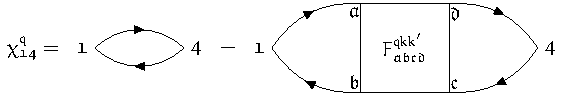
\includegraphics[scale=1.2]{../../Graphics/Diagrams/physical_susceptibility/physical_susceptibility}
	\caption{The physical susceptibility is defined as the generalized susceptibility with contracted legs, see \eqref{eq:phys_susc_contracted_legs}.}
	\label{fig:physical_susceptibility}
\end{figure}
Similarly, the contracted bubble susceptibility can be written as
\begin{align}
	\chi_{0;\mathfrak{14}}^{\q}=\sum_{\k\kp;\mathfrak{23}}\chi_{0;\mathfrak{1234}}^{\q\k\kp}.
\end{align}
Analogously to \eqref{eq:two_particle_green_density} and \eqref{eq:two_particle_green_magnetic}, one can write down density and magnetic spin combinations of the physical susceptibility,
\begin{subequations}
\begin{align}
	\chi_{\dens}^{\q}&=\chi_{\uparrow\uparrow}^{\q}+\chi_{\uparrow\downarrow}^{\q}\qqand\label{eq:chi_dens}\\
	\chi_{\magn}^{\q}&=\chi_{\uparrow\uparrow}^{\q}-\chi_{\uparrow\downarrow}^{\q}=\chi_{\overline{\uparrow\downarrow}}^{\q}.\label{eq:chi_magn}
\end{align}
\end{subequations}
Note that expressions \eqref{eq:chi_dens} and \eqref{eq:chi_magn} are nothing more than the Fourier-transformed versions of \eqref{eq:chi_dens_derivative} and \eqref{eq:chi_magn_derivative}, respectively.

\section{Bethe-Salpeter equation}\label{sec:bethe_salpeter}

In the section above we have specified $\Gamma_{\r;\mathfrak{1234}}^{\q\k\kp}$ as the fully irreducible vertex in channel $\r$ and $\Phi_{\r;\mathfrak{1234}}^{\q\k\kp}$	as the reducible diagrams in channel $\r$. We can now construct the full set of $\Phi_{\r;\mathfrak{1234}}^{\q\k\kp}$ from the irreducible vertex by chaining them together with pairs of Green's functions connecting two irreducible vertices. This results in so-called ladders, 
\begin{subequations}\label{eq:ladder_phi_gamma}
\begin{align}
\begin{split}
	\Phi_{\r;\mathfrak{1234}}^{\q\k\kp}&=\sum_{\k_1;\mathfrak{abcd}} \Gamma_{\r;\mathfrak{12ab}}^{\q\k\k_1} G_{\mathfrak{bc}}^{\k_1} G_{\mathfrak{da}}^{\k_1-\q} \Gamma_{\r;\mathfrak{cd34}}^{\q\k_1\kp}\\
	&\quad+\sum_{\substack{\k_1\k_2;\mathfrak{abcd}\\\mathfrak{efgh}}} \Gamma_{\r;\mathfrak{12ab}}^{\q\k\k_1} G_{\mathfrak{bc}}^{\k_1} G_{\mathfrak{da}}^{\k_1-\q} \Gamma_{\r;\mathfrak{cdef}}^{\q\k_1\k_2} G_{\mathfrak{fg}}^{\k_2} G_{\mathfrak{he}}^{\k_2-\q} \Gamma_{\r;\mathfrak{gh34}}^{\q\k_2\kp} + \dots
\end{split}\\
\begin{split}
	&=-\frac1\beta\sum_{\k_1;\mathfrak{abcd}} \Gamma_{\r;\mathfrak{12ab}}^{\q\k\k_1} \chi^{\q\k_1\k_1}_{0;\mathfrak{badc}} \Gamma_{\r;\mathfrak{cd34}}^{\q\k_1\kp}\\
	&\phantom{-}\quad+\frac{1}{\beta^2}\sum_{\substack{\k_1\k_2;\mathfrak{abcd}\\\mathfrak{efgh}}} \Gamma_{\r;\mathfrak{12ab}}^{\q\k\k_1} \chi^{\q\k_1\k_1}_{0;\mathfrak{badc}} \Gamma_{\r;\mathfrak{cdef}}^{\q\k_1\k_2} \chi^{\q\k_2\k_2}_{0;\mathfrak{fehg}} \Gamma_{\r;\mathfrak{gh34}}^{\q\k_2\kp} + \dots
\end{split}
\end{align}
\end{subequations}
By combining \eqref{eq:full_vertex_gamma_phi} and \eqref{eq:ladder_phi_gamma}, one can obtain the Bethe-Salpeter equation (BSE) in all three channels \cite{a relativistic equation for bound-state, nambu paper, rohringer thesis maybe},
\begin{subequations}\label{eq:bethe_salpeter_vertex_three_channels}
\begin{align}
	F_{\mathfrak{1234}}^{\q\k\kp}&=\Gamma_{\ph;\mathfrak{1234}}^{\q\k\kp}-\frac1\beta\sum_{\k_1\k_2;\mathfrak{abcd}} \Gamma_{\ph;\mathfrak{12ba}}^{\q\k\k_1} \chi_{0;\mathfrak{abcd}}^{\q\k_1\k_2} F_{\ph;\mathfrak{dc34}}^{\q\k_2\kp}\\
	&=\Gamma_{\phbar;\mathfrak{1234}}^{\q\k\kp}+\frac1\beta\sum_{\k_1\k_2;\mathfrak{abcd}} \Gamma_{\phbar;\mathfrak{12ba}}^{\q\k\k_1} \chi_{0;\mathfrak{abcd}}^{\q\k_1\k_2} F_{\phbar;\mathfrak{dc34}}^{\q\k_2\kp}\\
	&=\Gamma_{\pp;\mathfrak{1234}}^{\q\k\kp}-\frac{1}{2\beta}\sum_{\k_1\k_2;\mathfrak{abcd}} \Gamma_{\pp;\mathfrak{12ba}}^{\q\k\k_1} \chi_{0;\mathfrak{abcd}}^{\q\k_1\k_2} F_{\pp;\mathfrak{dc34}}^{\q\k_2\kp},
\end{align}
\end{subequations}
where we have expressed the full vertex $F_{\mathfrak{1234}}^{\q\k\kp}$ in terms of the irreducible vertex $\Gamma_{\r;\mathfrak{1234}}^{\q\k\kp}$ and the generalized (bubble) susceptibility as a Dyson-like equation. Note that for \eqref{eq:bethe_salpeter_vertex_three_channels} we used the same channel reducibility and frequency notation for each separate line. This results in a key property of the BSE: the equation becomes diagonal in the bosonic transfer momentum and frequency $\q$. This can be taken advantage of in numerical computations as it makes it especially easy to parallelize over $\q$ as it is independent of all other quantum numbers. If we had not chosen the channel reducibility equal to the frequency notation, then the new $\q'$ would depend on the fermionic frequencies (the precise dependency is channel-specific, but in general $\q'=f(\q,\k,\kp)$) and the transformed BSE would not be diagonal in $\q'$. 

\eqref{eq:bethe_salpeter_vertex_three_channels} can be rewritten in terms of susceptibilities with the help of \eqref{eq:generalized_susceptibility},
\begin{subequations}\label{eq:bethe_salpeter_susc}
\begin{align}
	\chi^{\q\k\kp}_{\mathfrak{1234}}&=\chi^{\q\k\kp}_{0;\mathfrak{1234}}-\frac{1}{\beta^2}\sum_{\k_1\k_2;\mathfrak{abcd}}\chi^{\q\k\k_1}_{0;\mathfrak{12ba}} \Gamma^{\q\k_1\k_2}_{\ph;\mathfrak{abcd}} \chi^{\q\k_2\kp}_{\ph;\mathfrak{dc34}}\\
	&=\chi^{\q\k\kp}_{0;\mathfrak{1234}}+\frac{1}{\beta^2}\sum_{\k_1\k_2;\mathfrak{abcd}}\chi^{\q\k\k_1}_{0;\mathfrak{12ba}} \Gamma^{\q\k_1\k_2}_{\phbar;\mathfrak{abcd}} \chi^{\q\k_2\kp}_{\phbar;\mathfrak{dc34}}\\
	&=\chi^{\q\k\kp}_{0;\mathfrak{1234}}-\frac{1}{2\beta^2}\sum_{\k_1\k_2;\mathfrak{abcd}}\chi^{\q\k\k_1}_{0;\mathfrak{1c3a}}\Gamma^{\q\k_1\k_2}_{\pp;\mathfrak{abcd}}\left (\chi^{\q\k_2\kp}_{\pp;\mathfrak{d2b4}}+\chi^{\q\k_2\kp}_{0;\mathfrak{d2b4}}\right )\label{eq:bethe_salpeter_susc_pp}.
\end{align}
\end{subequations}
This is the most general form of the Bethe-Salpeter equations, where energy and momentum is conserved. If the system under consideration is additionally SU(2)-symmetric, then we can formulate the BSE in terms of density and magnetic spin components,
\begin{subequations}
\begin{align}
	F_{\dens/\magn;\ph;\mathfrak{1234}}^{\q\k\kp}&=\Gamma_{\dens/\magn;\ph;\mathfrak{1234}}^{\q\k\kp}-\frac1\beta\sum_{\k_1\k_2;\mathfrak{abcd}} \Gamma_{\dens/\magn;\ph;\mathfrak{12ba}}^{\q\k\k_1} \chi_{0;\mathfrak{abcd}}^{\q\k_1\k_2} F_{\dens/\magn;\ph;\mathfrak{dc34}}^{\q\k_2\kp}\qqand\\
	F_{\dens/\magn;\phbar;\mathfrak{1234}}^{\q\k\kp}&=\Gamma_{\dens/\magn;\phbar;\mathfrak{1234}}^{\q\k\kp}-\frac1\beta\sum_{\k_1\k_2;\mathfrak{abcd}} \Gamma_{\dens/\magn;\phbar;\mathfrak{12ba}}^{\q\k\k_1} \chi_{0;\mathfrak{abcd}}^{\q\k_1\k_2} F_{\dens/\magn;\phbar;\mathfrak{dc34}}^{\q\k_2\kp}.
\end{align}
\end{subequations}
Likewise, the BSE decouples for other spin-symmetric combinations in for the pp-channel. These are the (s)inglet and (t)riplet channel, where
\begin{align}
	F_{\sing;\pp;\mathfrak{1234}}^{\q\k\kp}&=\Gamma_{\sing;\pp;\mathfrak{1234}}^{\q\k\kp}+\frac{1}{2\beta}\sum_{\k_1\k_2;\mathfrak{abcd}} \Gamma_{\sing;\pp;\mathfrak{12ba}}^{\q\k\k_1} \chi_{0;\mathfrak{abcd}}^{\q\k_1\k_2} F_{\sing;\pp;\mathfrak{dc34}}^{\q\k_2\kp}\qqand\\
	F_{\trip;\pp;\mathfrak{1234}}^{\q\k\kp}&=\Gamma_{\trip;\pp;\mathfrak{1234}}^{\q\k\kp}-\frac{1}{2\beta}\sum_{\k_1\k_2;\mathfrak{abcd}} \Gamma_{\trip;\pp;\mathfrak{12ba}}^{\q\k\k_1} \chi_{0;\mathfrak{abcd}}^{\q\k_1\k_2} F_{\trip;\pp;\mathfrak{dc34}}^{\q\k_2\kp}.
\end{align}
For a visual representation of the Bethe-Salpeter equation (\ref{eq:bethe_salpeter_vertex_three_channels}), see \figref{fig:bethe_salpeter_diagrammatic}.
\begin{figure}[ht!]
  \centering
  \parbox{\textwidth}{
    \subfloat{\includestandalone[scale=0.94]{../../Graphics/Diagrams/bse/bse_separate_ph}}
  }\\[1cm]
  \parbox{\textwidth}{
    \subfloat{\includestandalone[scale=0.94]{../../Graphics/Diagrams/bse/bse_separate_ph_bar}}
  }\\[1cm]
  \parbox{\textwidth}{
    \subfloat{\includestandalone[scale=0.94]{../../Graphics/Diagrams/bse/bse_separate_pp}}
  }
  \caption{Diagrammatic version of the BSE in all three channels for arbitrary spin components, see \eqref{eq:bethe_salpeter_vertex_three_channels}. The lower legs are exchanged in pp-notation, hence their direction is reversed.}
  \label{fig:bethe_salpeter_diagrammatic}
\end{figure}
The BSE of \eqref{eq:bethe_salpeter_vertex_three_channels} needs to be inverted in order to be able to yield the full vertex $F_{\mathfrak{1234}}^{\q\k\kp}$. This can be done in a smart way by viewing the multiplications of the vertex functions in the BSE as matrix multiplications written down in grouped indices. This means that for each transfer momentum $\q$, we can generate a matrix from a vertex by grouping the left (right) two orbital indices and fermionic frequencies into a new grouped index $n=\{n_1, n_2, \k\}$ ($m=\{n_3, n_4, \kp\}$), such that \cite{ab initio dyn} 
\begin{align}
	\bm{F}^{\q}_{\text{nm}}=F^{\q\k\kp}_{\mathfrak{1234}}.
\end{align}
This allows for a straightforward numerical implementation of vertex products and inversions with respect to these grouped indices. Hence, this yields for the full vertex $\bm{F}^{\q}_{\dens/\magn;\text{nm}}$ obtained from the BSE,
\begin{align}
	\bm{F}^{\q}_{\dens/\magn;\text{nm}}=\left (\unity_{\text{nm}} +\frac1\beta \bm{\Gamma}^{\q}_{\dens/\magn;\text{nl}}\bm{\chi}^{\q}_{0;\text{lm}}\right )^{-1}.
\end{align}

\section{Schwinger-Dyson equation}\label{sec:schwinger_dyson}

To fill the missing gap in our (almost) complete theory of correlated electrons on a lattice, we have to consider the calculation of the self-energy which enters the many-body Green's function through \eqref{eq:dyson_eq}. This is done by the Schwinger-Dyson equation, which is derived as an equation of motion for the self-energy \cite{rohringer thesis} and connects the self-energy to the full vertex via\footnote{In its most general form, the self-energy $\Sigma$ also depends on the particle spin $\sigma$. In the SU(2)-symmetric case however we can omit the spin label, since $\Sigma_{\uparrow}=\Sigma_{\downarrow}=\Sigma$.} \cite{anna galler thesis, ab initio dga}
\begin{align*}
	\Sigma_{\mathfrak{12}}^{\k}&=\Sigma_{\text{HF};\mathfrak{12}}^{\vv{k}}+\Sigma_{\mathfrak{12}}^{\text{conn};\k}\\
	&=\!\underbrace{2\sum_{\mathfrak{ab};\vv{k}'}\!\mathcal{U}^{\vv{q}=\vv{0}}_{\mathfrak{12ab}}n_{\mathfrak{ba}}^{\vv{k}'}-\sum_{\mathfrak{ab},\vv{q}}\mathcal{U}^{\vv{q}}_{\mathfrak{1ba2}}n_{\mathfrak{ba}}^{\vv{k}-\vv{q}}}_{\Sigma_{\text{HF};\mathfrak{12}}^{\vv{k}}}\underbrace{-\frac1\beta\sum_{\substack{\mathfrak{abcdef}\\\q\kp}}\mathcal{U}^{\vv{q}}_{\mathfrak{a1bc}}\chi_{0;\mathfrak{cbed}}^{\q\kp\kp}F_{\mathfrak{de2f}}^{\q\kp\k}G_{\mathfrak{af}}^{\k-\q}}_{\Sigma_{\mathfrak{12}}^{\text{conn};\k}}\numberthis\label{eq:sde},
\end{align*}
where the first two sums in \eqref{eq:sde} are coined Hartree- and Fock-terms, respectively, and the third term is the vertex part and only contains connected diagrams. A visual representation of the Schwinger-Dyson equation can be seen in \figref{fig:sde}. 
\begin{figure}[ht!]
	\centering
  	\includestandalone[scale=1]{../../Graphics/Diagrams/sde/sde}
  	\caption{Representation of the Schwinger-Dyson equation (\ref{eq:sde}).}
  	\label{fig:sde}
\end{figure}
The $\ph$ and $\phbar$ contributions of the connected part yield separately (in ph notation)\footnote{With the help of \eqref{eq:phi_ph_bar_dens_magn}} \cite{ab initio dga}
\begin{subequations}
\begin{align}
	\Sigma^{\text{conn};\k}_{\ph;\mathfrak{12}}&=-\frac1\beta\sum_{\substack{\mathfrak{abcdef}\\\q\kp}}\mathcal{U}^{\vv{q}}_{\mathfrak{a1bc}}\chi^{\q\kp\kp}_{0;\mathfrak{cbed}}F^{\q\kp\k}_{\dens;\mathfrak{de2f}}G_{\mathfrak{af}}^{\k-\q}\qqand\\
	\Sigma^{\text{conn};\ph;\k}_{\phbar;\mathfrak{12}}&=-\frac{1}{2\beta}\sum_{\substack{\mathfrak{abcdef}\\\q\kp}}\tilde{\mathcal{U}}^{\vv{k}'-\vv{k}}_{\mathfrak{a1bc}}\chi^{\q\kp\kp}_{0;\mathfrak{cbed}}\left [F^{(\kp-\k)(\kp-\q)\kp}_{\dens;\mathfrak{2edf}}+3 F^{(\kp-\k)(\kp-\q)\kp}_{\magn;\mathfrak{2edf}}\right ]G_{\mathfrak{af}}^{\k-\q}.
\end{align}
\end{subequations}
The self-energy $\Sigma^{\k}_{\mathfrak{12}}$ does not have to fulfill any crossing-symmetry relation, hence we do not use $\mathcal{U}^{\vv{qkk}'}_{\mathfrak{1234};\ss'}$ from \eqref{eq:crossing_symmetric_uq} here but rather the two terms with $\mathcal{U}$ and $\tilde{\mathcal{U}}$ separately. The total self-energy is now the sum of the Hartree-Fock contribution and the $\ph/\phbar$ terms. We want to note that the Schwinger-Dyson equation can be rewritten in terms of three-leg vertices (also commonly called Hedin-vertices) instead of four-point Green's functions, see \cite{hedin, krien boson exchange} to eliminate the need of calculating the full vertex $F$ via an inversion of the irreducible vertex $\Gamma$\footnote{In principle, one could retrieve the full vertex as $\bm F_{\r}^{\q}=\left [(\bm\Gamma_{\r}^{\q})^{-1}-\bm\chi_{0}^{\q}\right ]^{-1}$. However, as shown in Ref. \cite{schäfer nonperturbative}, the (local) irreducible vertex $\Gamma$ contains an infinite set of divergencies, hence inverting it is numerically unstable.}. This equivalent formulation is commonly called the Hedin form. In this form, the SDE can be rewritten in terms of suceptibilities. We start by rewriting the full vertex as a combination of susceptibilities
\begin{align}
	F^{\q\k\kp}_{\mathfrak{1234};\ss'}=\beta^2\left [\left (\chi_{0;\mathfrak{1234}}^{\q\k\kp}\right )^{-1}-\sum_{\k_1\k_2;\mathfrak{abcd}}\left (\chi_{0;\mathfrak{12ba}}^{\q\k\k_1}\right )^{-1} \chi_{\mathfrak{abcd};\ss'}^{\q\k_1\k_2} \left (\chi_{0;\mathfrak{dc34}}^{\q\k_2\kp}\right )^{-1}\right ]^{-1}.
\end{align}
Here and in the following, we will restrict ourselves to the $\ph$ channel reducibility and frequency notation if not stated otherwise. Next, we define the irreducible vertex as the first-order contribution - which is the bare Coulomb interaction in crossing-symmetric notation, see \eqref{eq:crossing_symmetric_uq} - and the rest,
\begin{align}
	\Gamma_{\mathfrak{1234};\ss'}^{\q\k\kp} = \mathcal{U}^{\vv{qkk}'}_{\mathfrak{1234};\ss'}+\delta\Gamma_{\mathfrak{1234};\ss'}^{\q\k\kp}.
\end{align}
It is then straightforward to define an auxiliary susceptibility (denoted by the asterisk $^*$)
\begin{align}
\begin{split}\label{eq:chi_aux}
	\chi_{\mathfrak{1234};\ss'}^{*;\q\k\kp}&=\left [\left (\chi_{0;\mathfrak{1234}}^{\q\k\k}\right )^{-1}+\frac{1}{\beta^2}\delta\Gamma_{\mathfrak{1234};\ss'}^{\q\k\kp}\right ]^{-1}\\
	&=\left [\left (\chi_{0;\mathfrak{1234}}^{\q\k\k}\right )^{-1}+\frac{1}{\beta^2}\left (\Gamma_{\mathfrak{1234};\ss'}^{\q\k\kp}-\mathcal{U}^{\vv{qkk}'}_{\mathfrak{1234};\ss'}\right )\right ]^{-1},
\end{split}
\end{align}
with which we can rewrite the generalized susceptibility as
\begin{align}\label{eq:bse_susceptibilities}
	\chi_{\mathfrak{1234};\ss'}^{\q\k\kp}=\chi_{\mathfrak{1234};\ss'}^{*;\q\k\kp}-\sum_{\k_1\k_2;\mathfrak{abcd}}\chi_{\mathfrak{12ba};\ss'}^{*;\q\k\k_1}\, \mathcal{U}^{\vv{qk}_1\vv{k}_2}_{\mathfrak{abcd};\ss'} \chi_{\mathfrak{dc34};\ss'}^{\q\k_2\kp}.
\end{align}
Previously, the BSE was formulated as a ladder with $\Gamma_{\mathfrak{1234}}^{\q\k\kp}$ and $\chi_{0;\mathfrak{1234}}^{\q\k\k}$ as building blocks. The rewritten BSE can now be understood as a ladder with $\chi_{\mathfrak{1234};\ss'}^{*;\q\k\kp}$ and $\mathcal{U}^{\vv{qkk}'}_{\mathfrak{1234};\ss'}$ as building blocks. Here, the auxiliary susceptibility can be seen as the irreducible part with respect to the bare Coulomb interaction, contrary to how $\Gamma_{\mathfrak{1234}}^{\q\k\kp}$ is the set of irreducible diagrams with respect to cutting two Green function lines (or a bare susceptibility $\chi_{0;\mathfrak{1234}}^{\q\k\k}$). Hence, this is commonly called interaction-reducibility \cite{krien single boson}. The BSE displayed in terms of susceptibilities can be seen in \figref{fig:bse_susceptibilities}.
\begin{figure}[ht!]
	\centering
  	\includestandalone[width=\textwidth]{../../Graphics/Diagrams/bse_susceptibilities/bse_susceptibilities}
  	\caption{Interaction-reducible form of the Schwinger-Dyson equation (\ref{eq:bse_susceptibilities}) with susceptibilities.}
  	\label{fig:bse_susceptibilities}
\end{figure}
If one neglects the nonlocal $\phbar$ contribution from the bare Coulomb interaction, one can rewrite the following expression in terms of sums of susceptibilities, where after some algebra,
\begin{align}
	\sum_{\kp;\mathfrak{ab}}F_{\mathfrak{12ab};\ss'}^{\q\k\kp}\chi_{0;\mathfrak{ba34}}^{\q\kp\kp}=\beta\sum_{\mathfrak{abcd};\sigma_1}\gamma_{\mathfrak{12ab};\ss'}^{\q\k}\!\left (\unity_{\mathfrak{ba34}}^{\k\kp}-\mathcal{U}^{\vv{q}}_{\mathfrak{badc};\ss_1}\chi^{\q}_{\mathfrak{cd34};\sigma_1\sigma}\right ),
\end{align}
where the Fermi-Bose three-leg vertex $\gamma_{\mathfrak{1234};\ss'}^{\q\k}$ is defined as
\begin{align}\label{eq:vrg}
	\gamma_{\mathfrak{1234};\ss'}^{\q\k} = \beta \sum_{\k_1;\mathfrak{ab}}\left (\chi_{0;\mathfrak{12ab}}^{\q\k\k}\right )^{-1}\chi_{\mathfrak{ba34};\ss'}^{*;\q\k\k_1}.
\end{align}
This allows us to rewrite \eqref{eq:sde} as
\begin{align}\label{eq:sde_vrg}
	\Sigma_{\mathfrak{12};\ss'}^{\k}=\Sigma_{\text{HF};\mathfrak{12}}^{\vv{k}}-\sum_{\substack{\q;\mathfrak{abcd}\\\mathfrak{efgh};\sigma_1}}\mathcal{U}^{\vv{q}}_{\mathfrak{a1bc}}\left [\gamma_{\mathfrak{aced};\ss'}^{\q\k}\big (\unity_{\mathfrak{deh2}}-\mathcal{U}^{\vv{q}}_{\mathfrak{defg};\ss_1}\chi_{\mathfrak{gfh2};\sigma_1\sigma'}^{\q}\big)\right ]G_{\mathfrak{bh}}^{\k-\q}.
\end{align}
A visual representation of the rewritten SDE can be found in \figref{fig:sde_vrg}. 
\begin{figure}[ht!]
	\centering
  	\includestandalone[scale=1]{../../Graphics/Diagrams/sde_vrg/sde_vrg}
  	\caption{Interaction-reducible form of the Schwinger-Dyson equation (\ref{eq:sde_vrg}) with three-leg vertices.}
  	\label{fig:sde_vrg}
\end{figure}
This expression has some numerical advantages, since the frequency dimensions of the Fermi-Bose vertices needed for the calculation of the self-energy are by one smaller compared to the approach with the full vertices, hence reducing the required memory storage in the process. 
\\\\
For numerical calculations of the equations in the above sections one is always restricted to a certain frequency range where the input quantities are known, which is usually limited by time and the impurity solver's capabilities. However, the full and irreducible vertex functions outside of this \say{core} frequency box are often not negligible\footnote{Especially not if one is interested in low-temperature behavior. Since the frequencies scale with $\sim\frac1\beta\sim T$, the smaller the temperature, the smaller the effective frequency box. Even though the full and irreducible vertex functions decay like $\frac{1}{\nu}$ as $\nu\to\infty$, the contributions outside of the core frequency region are of importance.}. Hence for more accurate descriptions of materials, one employs explicit asymptotics that should mimic the outer frequency structure of the vertex functions. These asymptotics can be done in many ways, from the simple concatenation of constant values\footnote{Like the bare Coulomb interaction $\mathcal{U}^{\vv{qkk}'}_{\mathfrak{1234};\ss'}$} to more complicated formulations using so-called kernel functions. In this thesis we want to introduce two treatments of asymptotic behavior in vertex functions: one being the kernel-function approach, where upon the pioneering work of Ref. \cite{kunes} and subsequent development of a full local framework \cite{wentzell, tagliavini, hummel, qmc asympt, kaufmann da} has been developed that mimics the coarse frequency structure of the vertex function outside of the core frequency region; and the other being an \say{RPA-esque} approach \cite{motoharu asympt}, where a constant value outside the core frequency region of the irreducible vertex is assumed and diagrams are generated by a ladder, similar to the BSE. We will outline the two methods in detail, explain their advantages and drawbacks and reason briefly when to choose either of them. Since the former method using kernel-functions has not been generalized to non-local quantities yet at the writing of this thesis, we will derive equations that include non-local contributions to better incorporate these asymptotics in the upcoming frameworks that will be introduced. 

\section{Vertex asymptotics}\label{sec:vertex_asymptotics}

A full treatment of frequency and momentum dependence of multi-orbital vertex functions severely restricts the speed and memory consumption of numerical calculations. A step towards reducing the computational cost of numerical implementations of equations involving vertex functions, such as the Bethe-Salpeter equations, see \secref{sec:bethe_salpeter}, or the Schwinger-Dyson equation, see \secref{sec:schwinger_dyson}, thus requires an efficient treatment of the vertex for high Matsubara frequencies. As noted above, we will describe two treatments of vertex asymptotics in the following.

\subsection{Kernel-function asymptotics}\label{sec:vertex_asymptotics_kernel}

Shortly, we will see, that the full vertex in the high-frequency regime, which generally depends on three independent frequency parameters, can be approximated well as an object with only two frequency dimensions, thus drastically reducing the storage capacity required, while also reducing the computational cost after assembling these objects. Let us start with a sketch of the basic idea of how to take advantage of certain frequency structures when handling explicit vertex asymptotics.
\begin{figure}[ht!]
	\centering
	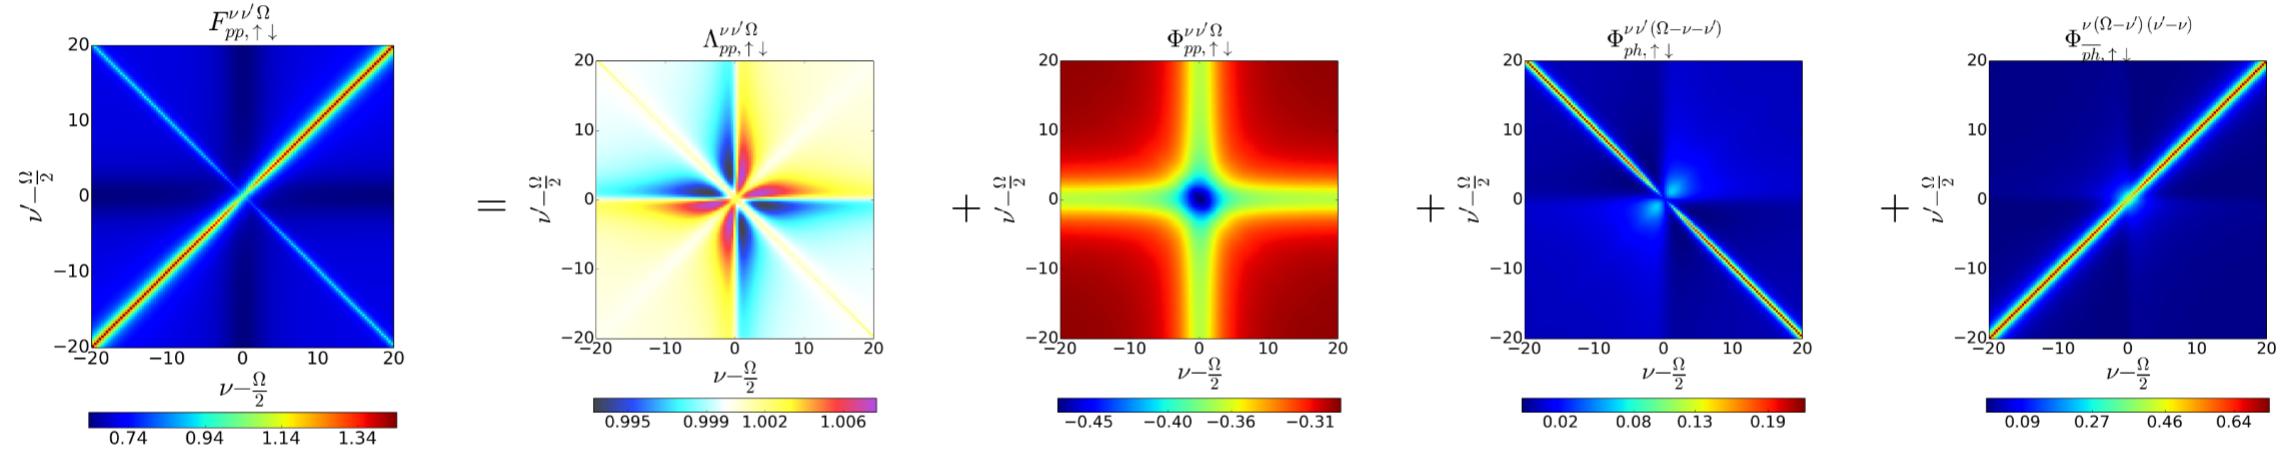
\includegraphics[width=\linewidth]{../../Graphics/vertex_asymptotics_paper.png}
	\caption{Numerical SIAM results for all local vertices contained in the parquet equation \eqref{eq:parquet_decomposition} for vanishing transfer frequency $\Omega=0$, taken from Ref. \cite{high-freq asympt}. In our convention, $\Omega$ should be replaced by $\omega$.}
	\label{fig:full_vertex_siam_results_paper}
\end{figure}
In \figref{fig:full_vertex_siam_results_paper}, the frequency dependence of local vertex functions $F^{\omega\nu\nu'}_{\pp;\uparrow\downarrow}$, $\Lambda^{\omega\nu\nu'}_{\pp;\uparrow\downarrow}$ and $\Phi^{\omega\nu\nu'}_{\r;\uparrow\downarrow}$ calculated for the Single-Impurity Anderson Model (SIAM) are shown for vanishing transfer frequency $\omega$ \cite{high-freq asympt}. From this, one can see three very prominent and distinct features of the full vertex $F$: (i) a constant background that differs from the (local and constant) Hubbard interaction $U$; (ii) two diagonal structures, the main ($\nu=\nu'$) and secondary ($\nu=-\nu'$) diagonal; and (iii) a \say{cross}-like structure along $\nu=\pm\frac\pi\beta$ and $\nu'=\pm\frac\pi\beta$. While only shown for the antiparallel spin combination $\uparrow\downarrow$ and vanishing transfer frequency $\omega=0$, the features are analogous for the parallel spin combination $\uparrow\uparrow$ and for finite $\omega\neq0$. These three attributes do \textit{not} decay for high Matsubara frequencies $\nu$ and $\nu'$ and therefore indicate complex asymptotic behaviour. The individual asymptotic contributions of the fully irreducible vertex $\Lambda$ and the reducible vertex in channel r to the full vertex $F$ are written in detail in Ref. \cite{high-freq asympt}. Summarized, $\Lambda$ adds a constant background of size $U$, $\Phi_{\ph}$ adds a secondary diagonal structure, $\Phi_{\phbar}$ adds a diagonal structure and $\Phi_{\pp}$ adds a constant background and a \say{cross}-like structure. Notice that the description in Ref. \cite{high-freq asympt} only refers to the SIAM model and considers solely the one-band case with local quantities and a constant local interaction $U$. An extension to a multi-orbital formalism and momentum-dependent vertices and interaction $U$ follows naturally and will be discussed shortly.

The simplest quantity to describe in terms of their asymptotics is the fully irreducible vertex $\Lambda^{\q\k\kp}_{\mathfrak{1234}}$, for which
\begin{align}
	\Lambda^{\asympt;\q\k\kp}_{\mathfrak{1234};\ss'}\approx\mathcal{U}^{\vv{qkk}'}_{\mathfrak{1234};\ss'},
\end{align}
where $\mathcal{U}^{\vv{qkk}'}_{\mathfrak{1234};\ss'}$ is the non-local Coulomb interaction, written in crossing-symmetric notation
\begin{align}\label{eq:crossing_symmetric_uq}
	 \mathcal{U}^{\vv{qkk}'}_{\mathfrak{1234};\ss'}=\underbrace{U_{\mathfrak{1234}}+V^{\vv{q}}_{\mathfrak{1234}}}_{\mathcal{U}^{\vv{q}}_{\mathfrak{1234}}}-\delta_{\ss'}\big (\underbrace{U_{\mathfrak{2314}}+V^{\vv{k}'-\vv{k}}_{\mathfrak{2314}}}_{\tilde{\mathcal{U}}^{\vv{k}'-\vv{k}}_{\mathfrak{1234}}}\big ),
\end{align}
containing the purely local interaction $U$ and the purely non-local interaction $V$. \eqref{eq:crossing_symmetric_uq} is diagrammatically displayed in \figref{fig:bare_vertex_crossing_symmetric}.
\begin{figure}[ht!]
	\centering
	\includestandalone[scale=1]{../../Graphics/Diagrams/bare_vertex_crossing_symmetric/bare_vertex_crossing_symmetric}
	\caption{Crossing-symmetric interaction, see \eqref{eq:crossing_symmetric_uq}.}
	\label{fig:bare_vertex_crossing_symmetric}
\end{figure}
Constructing $\dens,\magn,\sing$ and $\trip$ combinations of \eqref{eq:crossing_symmetric_uq} is useful for future calculations,
\begin{subequations}
\begin{align}
	\mathcal{U}^{\vv{qkk}'}_{\dens;\mathfrak{1234}}&=2\,\mathcal{U}^{\vv{q}}_{\mathfrak{1234}} - \tilde{\mathcal{U}}^{\vv{k}'-\vv{k}}_{\mathfrak{1234}},\\
	\mathcal{U}^{\vv{qkk}'}_{\magn;\mathfrak{1234}}&=-\tilde{\mathcal{U}}^{\vv{k}'-\vv{k}}_{\mathfrak{1234}},\\
	\mathcal{U}^{\vv{qkk}'}_{\sing;\mathfrak{1234}}&=\mathcal{U}^{\vv{k}+\vv{k}'-\vv{q}}_{\mathfrak{1234}}+\tilde{\mathcal{U}}^{\vv{k}'-\vv{k}}_{\mathfrak{1234}}\qqand\\
	\mathcal{U}^{\vv{qkk}'}_{\trip;\mathfrak{1234}}&=\mathcal{U}^{\vv{k}+\vv{k}'-\vv{q}}_{\mathfrak{1234}}-\tilde{\mathcal{U}}^{\vv{k}'-\vv{k}}_{\mathfrak{1234}}.
\end{align}
\end{subequations}
Next, we begin examining the diagrams contributing to $\Phi_{\r}$. A smart choice introduced in Ref. \cite{high-freq asympt} is to classify these diagrams in each channel further into three categories:
\begin{itemize}
	\item Class 1: These are diagrams which connect incoming and outgoing particles only by a single interaction vertex. These diagrams are bubble diagrams and hence only depend on a single bosonic frequency and momentum. The sum of all these diagrams will be encoded in the variable $\mathcal{K}^{(1);\q}_{\r;\mathfrak{1234};\ss'}$, see the first line in \figref{fig:kernel_functions}.
	\item Class 2: Diagrams corresponding to class 2 are identified by them having either the incoming \textit{or} outgoing particles connected to the same interaction vertex. These diagrams depend on the bosonic transfer frequency and momentum and one fermionic frequency and momentum. The sum of all these diagrams will be encoded in the variables $\mathcal{K}^{(2);\q\k}_{\r;\mathfrak{1234};\ss'}$ and $\overline{\mathcal{K}}^{(2);\q\k}_{\r;\mathfrak{1234};\ss'}$, depending on whether the outgoing particles ($\mathcal{K}$) or the incoming particles ($\overline{\mathcal{K}}$) are connected to the interaction vertex, see the second line in \figref{fig:kernel_functions}. $\mathcal{K}$ and $\overline{\mathcal{K}}$ are related to each other via time-reversal symmetry, where in the case of a system with additional SU(2)-symmetry corresponds to \cite{rohringer thesis} $\mathcal{K}^{(2);\q\k}_{\r;\mathfrak{1234};\ss'}=\overline{\mathcal{K}}^{(2);\q\k}_{\r;\mathfrak{1234};\ss'}$.
	\item Class 3: These are diagrams where each external Green's function is connected to a different interaction vertex. These diagrams are parametrized by three independent frequency and momentum arguments and are encoded in the \say{rest} function $\mathcal{R}^{\q\k\kp}_{\r;\mathfrak{1234};\ss'}$.
\end{itemize}
In the following, we will refer to $\mathcal{K}^{(1)}$, $\mathcal{K}^{(2)}$ and $\overline{\mathcal{K}}^{(2)}$ as kernel functions. One now can - with the help of these classifications - write the reducible $\Phi_{\r}$-vertices as a decomposition of the different kernel functions and the \say{rest}-function
\begin{align}
	\Phi_{\r;\mathfrak{1234};\ss'}^{\q\k\kp}=\mathcal{K}^{(1);\q}_{\r;\mathfrak{1234};\ss'}+\mathcal{K}^{(2);\q\k}_{\r;\mathfrak{1234};\ss'}+\mathcal{K}^{(2);\q\k'}_{\r;\mathfrak{1234};\ss'}+\mathcal{R}^{\q\k\kp}_{\r;\mathfrak{1234};\ss'}.
\end{align}
This composition is \textit{per se} exact. However, to take advantage of this formalism for numerical calculations, one discards the \say{rest}-function due to its additional frequency dependence entering the inner propagators, resulting in a quicker drop-off in all frequency directions. Thus, the approximation
\begin{align}\label{eq:asympt_phi_r}
	\Phi_{\r;\mathfrak{1234};\ss'}^{\asympt;\q\k\kp}\approx\mathcal{K}^{(1);\q}_{\r;\mathfrak{1234};\ss'}+\mathcal{K}^{(2);\q\k}_{\r;\mathfrak{1234};\ss'}+\mathcal{K}^{(2);\q\k'}_{\r;\mathfrak{1234};\ss'}
\end{align}
serves as a valid expression for the high-frequency regime of $\Phi_{\r}$ and becomes exact for $\nu,\nu'\to\infty$ \cite{high-freq asympt}. As we can see above, the quantities on the right hand side of \eqref{eq:asympt_phi_r} only depend on one ($\q$) or two ($\q,\k$) Matsubara frequencies and momenta instead of three, reducing the numerical complexity and memory usage for $\Phi_{\r}$ significantly. Using these explicit asymptotics results in a tremendous improvement of numerical results over a simple truncation in $\Phi_{\r}$ for high frequencies \cite{high-freq asympt}. The explicit expressions for the kernel functions needed to calculate the reducible diagrams can be obtained by \cite{towards ab initio dga, josef DA, pudleiner paper}
\begin{align}
 	\mathcal{K}^{(1);\q}_{\ph;\mathfrak{1234};\ss'}&=\!\!\!\sum_{\substack{\mathfrak{abcd};\k_1\k_2\\\sigma_1\sigma_2}} \!\!\!\mathcal{U}^{\vv{q}\vv{k}_1}_{\mathfrak{12ab};\ss_1}\chi^{\q\k_1\k_2}_{\mathfrak{badc};\sigma_1\sigma_2}\mathcal{U}^{\vv{q}(-\vv{k}_2)}_{\mathfrak{cd34};\sigma_2\sigma'},\label{eq:kernel_1}\\
 	\mathcal{K}^{(1);\q}_{\pp;\mathfrak{1234};\ss'}&=\frac14\!\!\!\sum_{\substack{\mathfrak{abcd};\k_1\k_2\\\sigma_1\sigma_2\sigma_3\sigma_4}} \!\!\!\mathcal{U}^{\vv{q}\vv{k}_1}_{\substack{\mathfrak{1b3a}\\\ss_2\sigma'\sigma_1}}\chi^{\q\k_1\k_2}_{\substack{\mathfrak{acbd}\\\sigma_1\sigma_3\sigma_2\sigma_4}}\mathcal{U}^{\vv{q}(-\vv{k}_2)}_{\substack{\mathfrak{d2c4}\\\sigma_4\sigma\sigma_3\sigma'}},\label{eq:kernel_1_pp}\\
\begin{split}\label{eq:kernel_2}
	\mathcal{K}^{(2);\q\k}_{\ph;\mathfrak{1234};\ss'}&=\sum_{\substack{\mathfrak{ab};\k_1\\\sigma_1}} F^{\q\k\k_1}_{\mathfrak{12ab};\ss_1}\,\chi^{\q\k_1\k_1}_{0;\mathfrak{baab}}\,\mathcal{U}^{\vv{q}(-\vv{k}_1)}_{\mathfrak{ba34};\sigma_1\sigma'}-\mathcal{K}^{(1);\q}_{\ph;\mathfrak{1234};\ss'}\\
	&=-\sum_{\substack{\mathfrak{ab};\k_1\\\sigma_1}} \frac{\chi^{\q\k\k_1}_{\mathfrak{cdab};\ss_1}}{G^{\k}_{\mathfrak{c1}}G^{\k-\q}_{\mathfrak{2d}}}\,\mathcal{U}^{\vv{q}(-\vv{k}_1)}_{\mathfrak{ba34};\sigma_1\sigma'}-\mathcal{K}^{(1);\q}_{\ph;\mathfrak{1234};\ss'}
\end{split}\\
\begin{split}\label{eq:kernel_2_pp}
	\mathcal{K}^{(2);\q\k}_{\pp;\mathfrak{1234};\ss'}&=\frac12\!\!\!\sum_{\substack{\mathfrak{ab};\k_1\\\sigma_1\sigma_2\sigma_3\sigma_4}} \!\!\!F^{\q\k\k_1}_{\substack{\pp;\mathfrak{1a3b}\\\sigma\sigma_1\sigma'\sigma_2}}\,\chi^{\q\k_1\k_1}_{0;\mathfrak{baab}}\,\mathcal{U}^{\vv{q}(-\vv{k}_1)}_{\substack{\mathfrak{b2a4}\\\sigma_2\sigma\sigma_1\sigma'}}-\mathcal{K}^{(1);\q}_{\pp;\mathfrak{1234};\ss'}\\
	&=-\frac12\!\!\!\sum_{\substack{\mathfrak{abcd};\k_1\\\sigma_1\sigma_2\sigma_3\sigma_4}}\!\!\! \frac{\chi^{\q\k\k_1}_{\substack{\pp;\mathfrak{cadb}\\\sigma\sigma_1\sigma'\sigma_2}}}{G^{\k}_{\mathfrak{1c}}G^{-\q}_{\mathfrak{3d}}}\,\mathcal{U}^{\vv{q}(-\vv{k}_1)}_{\substack{\mathfrak{b2a4}\\\sigma_2\sigma\sigma_1\sigma'}}-\mathcal{K}^{(1);\q}_{\pp;\mathfrak{1234};\ss'}
\end{split}
\end{align}
where the subtraction of $\mathcal{K}^{(1)}$ in the kernel-2 function is to account for double-counting of diagrams and $\mathcal{U}^{\vv{qk}'}_{\mathfrak{1234};\ss'}$ is obtained from \eqref{eq:crossing_symmetric_uq} by setting $\vv{k}=\vv{0}$. Both kernel functions are displayed diagrammatically for the ph-channel in \figref{fig:kernel_functions}.
\begin{figure}[ht!]
  \centering
  \subfloat{\includestandalone[scale=1]{../../Graphics/Diagrams/kernel_functions/kernel_1_ph}}\\[0.5cm]
  \hspace{-0.25cm}\subfloat{\includestandalone[scale=1]{../../Graphics/Diagrams/kernel_functions/kernel_2_ph}}
  \caption{Diagrammatic version of the kernel-1 and kernel-2 functions of \eqref{eq:kernel_1} and \eqref{eq:kernel_2}.}
  \label{fig:kernel_functions}
\end{figure}
The density and magnetic contributions to the kernel functions read\footnote{Remember, that for density and magnetic contributions, frequencies should be in $\ph$ notation whereas for (s)inglet and (t)riplet contributions, frequencies should be in $\pp$ notation.}
\begin{subequations}\label{eq:kernel_functions_dens_magn}
\begin{align}
	\mathcal{K}^{(1);\q}_{\dens;\mathfrak{1234}}&=\sum_{\substack{\mathfrak{abcd}\\\k_1\k_2}} \mathcal{U}^{\vv{q}\vv{k}_1}_{\dens;\mathfrak{12ab}} \chi^{\q\k_1\k_2}_{\dens;\mathfrak{badc}} \mathcal{U}^{\vv{q}(-\vv{k}_2)}_{\dens;\mathfrak{cd34}},\\
	\mathcal{K}^{(1);\q}_{\magn;\mathfrak{1234}}&=\sum_{\substack{\mathfrak{abcd}\\\k_1\k_2}} \mathcal{U}^{\vv{q}\vv{k}_1}_{\magn;\mathfrak{12ab}} \chi^{\q\k_1\k_2}_{\magn;\mathfrak{badc}} \mathcal{U}^{\vv{q}(-\vv{k}_2)}_{\magn;\mathfrak{cd34}},\\
\begin{split}
	\mathcal{K}^{(2);\q\k}_{\dens;\mathfrak{1234}}&=\sum_{\mathfrak{ab};\k_1} F^{\q\k\k_1}_{\dens;\mathfrak{12ab}}\,\chi^{\q\k_1\k_1}_{0;\mathfrak{baab}}\,\mathcal{U}^{\vv{q}(-\vv{k}_1)}_{\dens;\mathfrak{ba34}}-\mathcal{K}^{(1);\q}_{\dens;\mathfrak{1234}}\\
	&=-\sum_{\mathfrak{abcd};\k_1} \frac{\chi^{\q\k\k_1}_{\dens;\mathfrak{cdab}}}{G^{\k}_{\mathfrak{c1}}G^{\k-\q}_{\mathfrak{2d}}}\,\mathcal{U}^{\vv{q}(-\vv{k}_1)}_{\dens;\mathfrak{ba34}}-\mathcal{K}^{(1);\q}_{\dens;\mathfrak{1234}}\qqand
\end{split}\\
\begin{split}
	\mathcal{K}^{(2);\q\k}_{\magn;\mathfrak{1234}}&=\sum_{\mathfrak{ab};\k_1} F^{\q\k\k_1}_{\magn;\mathfrak{12ab}}\,\chi^{\q\k_1\k_1}_{0;\mathfrak{baab}}\,\mathcal{U}^{\vv{q}(-\vv{k}_1)}_{\magn;\mathfrak{ba34}}-\mathcal{K}^{(1);\q}_{\magn;\mathfrak{1234}}\\
	&=-\sum_{\mathfrak{abcd};\k_1} \frac{\chi^{\q\k\k_1}_{\magn;\mathfrak{cdab}}}{G^{\k}_{\mathfrak{c1}}G^{\k-\q}_{\mathfrak{2d}}}\,\mathcal{U}^{\vv{q}(-\vv{k}_1)}_{\magn;\mathfrak{ba34}}-\mathcal{K}^{(1);\q}_{\magn;\mathfrak{1234}}.
\end{split}
\end{align}
\end{subequations}
The $\sing/\trip$ combinations can be constructed analogously for the pp-channel (written in pp frequency notation):
\begin{subequations}\label{eq:kernel_functions_sing_trip}
\begin{align}
	\mathcal{K}^{(1);\q}_{\sing;\mathfrak{1234}}&=\frac14\sum_{\substack{\mathfrak{abcd}\\\k_1\k_2}} \mathcal{U}^{\vv{q}\vv{k}_1}_{\sing;\mathfrak{1b3a}} \chi^{\q\k_1\k_2}_{\sing;\mathfrak{acbd}} \mathcal{U}^{\vv{q}(-\vv{k}_2)}_{\sing;\mathfrak{d2c4}}\stackrel{(\ref{eq:generalized_susceptibility_pp_ssp})}{=}\frac12\sum_{\substack{\mathfrak{abcd}\\\k_1\k_2}} \mathcal{U}^{\vv{q}\vv{k}_1}_{\sing;\mathfrak{1b3a}} \chi^{\pp;\q\k_1\k_2}_{\mathfrak{acbd};\uparrow\downarrow} \mathcal{U}^{\vv{q}(-\vv{k}_2)}_{\sing;\mathfrak{d2c4}},\\
	\mathcal{K}^{(1);\q}_{\trip;\mathfrak{1234}}&=\frac14\sum_{\substack{\mathfrak{abcd}\\\k_1\k_2}} \mathcal{U}^{\vv{q}\vv{k}_1}_{\trip;\mathfrak{1b3a}} \chi^{\q\k_1\k_2}_{\trip;\mathfrak{acbd}} \mathcal{U}^{\vv{q}(-\vv{k}_2)}_{\trip;\mathfrak{d2c4}}\stackrel{(\ref{eq:generalized_susceptibility_pp_ssp})}{=}0,\\
\begin{split}
	\mathcal{K}^{(2);\q\k}_{\sing;\mathfrak{1234}}&=\frac12\sum_{\mathfrak{ab};\k_1} F^{\q\k\k_1}_{\sing;\mathfrak{1a3b}}\,\chi^{\q\k_1\k_1}_{0;\mathfrak{baab}}\,\mathcal{U}^{\vv{q}(-\vv{k}_1)}_{\sing;\mathfrak{b2a4}}-\mathcal{K}^{(1);\q}_{\sing;\mathfrak{1234}}\\
	&=-\frac12\sum_{\mathfrak{abcd};\k_1} \frac{\chi^{\q\k\k_1}_{\sing;\mathfrak{cadb}}}{G^{\k}_{\mathfrak{1c}}G^{-\q}_{\mathfrak{3d}}}\,\mathcal{U}^{\vv{q}(-\vv{k}_1)}_{\sing;\mathfrak{b2a4}}-\mathcal{K}^{(1);\q}_{\sing;\mathfrak{1234}}\\
	&\!\!\stackrel{(\ref{eq:generalized_susceptibility_pp_ssp})}{=}-\sum_{\mathfrak{abcd};\k_1} \frac{\chi^{\pp;\q\k\k_1}_{\mathfrak{cadb};\uparrow\downarrow}}{G^{\k}_{\mathfrak{1c}}G^{-\q}_{\mathfrak{3d}}}\,\mathcal{U}^{\vv{q}(-\vv{k}_1)}_{\sing;\mathfrak{b2a4}}-\mathcal{K}^{(1);\q}_{\sing;\mathfrak{1234}}\qqand
\end{split}\\
\begin{split}
	\mathcal{K}^{(2);\q\k}_{\trip;\mathfrak{1234}}&=\frac12\sum_{\mathfrak{ab};\k_1} F^{\q\k\k_1}_{\trip;\mathfrak{1a3b}}\,\chi^{\q\k_1\k_1}_{0;\mathfrak{baab}}\,\mathcal{U}^{\vv{q}(-\vv{k}_1)}_{\trip;\mathfrak{b2a4}}-\mathcal{K}^{(1);\q}_{\trip;\mathfrak{1234}}\\
	&=-\frac12\sum_{\mathfrak{abcd};\k_1} \frac{\chi^{\q\k\k_1}_{\trip;\mathfrak{cadb}}}{G^{\k}_{\mathfrak{1c}}G^{-\q}_{\mathfrak{3d}}}\,\mathcal{U}^{\vv{q}(-\vv{k}_1)}_{\trip;\mathfrak{b2a4}}-\mathcal{K}^{(1);\q}_{\trip;\mathfrak{1234}}\stackrel{(\ref{eq:generalized_susceptibility_pp_ssp})}{=}0.
\end{split}
\end{align}	
\end{subequations}
Finally, the asymptotic part of the full vertex $\left (F_{\r;\mathfrak{1234};\ss'}^{\asympt;\q\k\kp}\right )$ can now be assembled using the asymptotic contributions of $\Lambda^{\asympt;\q\k\kp}_{\mathfrak{1234};\ss'}$ and $\Phi_{\r;\mathfrak{1234};\ss'}^{\asympt;\q\k\kp}$ through the parquet decomposition of \eqref{eq:parquet_decomposition}. This results in
\begin{align}
\begin{split}
	F_{\mathfrak{1234};\ss'}^{\asympt;\q\k\kp}-\;\mathcal{U}^{\vv{qkk}'}_{\mathfrak{1234};\ss'}&=\Phi_{\ph;\mathfrak{1234};\ss'}^{\asympt;\q\k\kp}+\Phi_{\phbar;\mathfrak{1234};\ss'}^{\asympt;\q\k\kp}+\Phi_{\pp;\mathfrak{1234};\ss'}^{\asympt;\q\k\kp},
\end{split}
\end{align}
or explicitly with kernel-1 and kernel-2 functions,
\begin{equation}
\begin{alignedat}{4}
	F_{\mathfrak{1234};\ss'}^{\asympt;\q\k\kp}-\;\mathcal{U}^{\vv{qkk}'}_{\mathfrak{1234};\ss'}=&\phantom{+}\;\,\mathcal{K}^{(1);\q}_{\ph;\mathfrak{1234};\ss'} &&+ \mathcal{K}^{(2);\q\k}_{\ph;\mathfrak{1234};\ss'}&&+\mathcal{K}^{(2);\q\k'}_{\ph;\mathfrak{1234};\ss'}\\
	&+\mathcal{K}^{(1);\q}_{\phbar;\mathfrak{1234};\ss'} &&+ \mathcal{K}^{(2);\q\k}_{\phbar;\mathfrak{1234};\ss'}&&+\mathcal{K}^{(2);\q\k'}_{\phbar;\mathfrak{1234};\ss'}\\
	&+\mathcal{K}^{(1);\q}_{\pp;\mathfrak{1234};\ss'} &&+ \mathcal{K}^{(2);\q\k}_{\pp;\mathfrak{1234};\ss'}&&+\mathcal{K}^{(2);\q\k'}_{\pp;\mathfrak{1234};\ss'}.
\end{alignedat}
\end{equation}
The asymptotic behavior of the irreducible vertex in channel r follows from \eqref{eq:full_vertex_gamma_phi},
\begin{align}
	\Gamma_{\r;\mathfrak{1234};\ss'}^{\asympt;\q\k\kp}&=F_{\mathfrak{1234};\ss'}^{\asympt;\q\k\kp}-\Phi_{\r;\mathfrak{1234};\ss'}^{\asympt;\q\k\kp}
\end{align}
and reads for the ph-channel explicitly
\begin{equation}
\begin{alignedat}{3}
	\Gamma_{\ph;\mathfrak{1234};\ss'}^{\asympt;\q\k\kp}&=\;\mathcal{U}^{\vv{qkk}'}_{\mathfrak{1234};\ss'}&&+\Phi_{\phbar;\mathfrak{1234};\ss'}^{\asympt;\q\k\kp}&&+\Phi_{\pp;\mathfrak{1234};\ss'}^{\asympt;\q\k\kp}\\
	&=\;\mathcal{U}^{\vv{qkk}'}_{\mathfrak{1234};\ss'}&&-\Phi_{\ph;\mathfrak{3214};\overline{\sigma'\sigma}}^{\asympt;(\kp-\k)(\kp-\q)\kp}&&+\Phi_{\pp;\mathfrak{1234};\ss'}^{\asympt;(\k+\kp-\q)\k\kp},
\end{alignedat}
\end{equation}
where we used \eqref{eq:phi_conversion_ph_bar_to_ph} to transform the $\phbar$-channel reducible vertex to a ph-channel reducible one. From this follows the irreducible vertex in the density and magnetic channel (in ph frequency notation) \cite{efficient BSE}
\begin{subequations}
\begin{equation}
\begin{alignedat}{3}
	\Gamma^{\asympt;\q\k\kp}_{\dens;\mathfrak{1234}}&=\;\mathcal{U}^{\vv{qkk}'}_{\dens;\mathfrak{1234}}&&-\frac12\Phi^{\asympt;(\kp-\k)(\kp-\q)\kp}_{\dens;\mathfrak{3214}}&&-\frac32\Phi^{\asympt;(\kp-\k)(\kp-\q)\kp}_{\magn;\mathfrak{3214}}\\
	&&&+\frac12\Phi_{\sing;\mathfrak{1234}}^{\asympt;(\k+\kp-\q)\k\kp}&&+\frac32\Phi_{\trip;\mathfrak{1234}}^{\asympt;(\k+\kp-\q)\k\kp},
\end{alignedat}
\end{equation}\\[-0.6cm]%
\begin{equation}
\begin{alignedat}{3}
	\Gamma^{\asympt;\q\k\kp}_{\magn;\mathfrak{1234}}&=\;\mathcal{U}^{\vv{qkk}'}_{\magn;\mathfrak{1234}} &&-\frac12\Phi^{\asympt;(\kp-\k)(\kp-\q)\kp}_{\dens;\mathfrak{3214}}&&+\frac12\Phi^{\asympt;(\kp-\k)(\kp-\q)\kp}_{\magn;\mathfrak{3214}}\\
	&&&-\frac12\Phi_{\sing;\mathfrak{1234}}^{\asympt;(\k+\kp-\q)\k\kp}&&+\frac12\Phi_{\trip;\mathfrak{1234}}^{\asympt;(\k+\kp-\q)\k\kp},
\end{alignedat}
\end{equation}
\end{subequations}
where the $\Phi_{\r;\mathfrak{1234}}^{\asympt;\q\k\kp}$ are given by the kernel functions of \eqref{eq:kernel_functions_dens_magn} and \eqref{eq:kernel_functions_sing_trip}. The irreducible vertices in channels $\phbar$ and $\pp$ in $\magn/\dens$ and $\sing/\trip$ combinations can be constructed analogously. 

\subsection{\text{$U$-range} asymptotics}\label{sec:vertex_asymptotics_urange}

Aside from the kernel-function formalism introduced above, there also exist many other asymptotic schemes for vertex functions. The second one we would like to cover in this thesis is the \say{$U$-range} approach, where the irreducible vertex $\Gamma_{\mathfrak{1234};\ss'}^{\q\k\kp}$ is padded with the bare non-local Coulomb interaction $\mathcal{U}^{\vv{qkk}'}_{\mathfrak{1234};\ss'}$, see \eqref{eq:crossing_symmetric_uq}, in the high-frequency regime. This in turn means that there is no complicated frequency structure for the asymptotic region. We denote some equations that are neccessary to employ these types of asymptotics and follow Ref. \cite{motoharu asympt} with the addition of multi-orbital notation. First, we will split up the frequencies into a \say{core} and an \say{asymptotic} region and denote quantities that exist in those frequency regimes with an additional sub- or superscript $\in\{\core, \asympt\}$. Generally speaking, we require $n_{\asympt}\ge n_{\core}$, where $n$ is the number of fermionic Matsubara frequencies. Furthermore, if a quantity is written as $(A^{\asympt})_\core$ it means that the asymptotic value of $A$ is cut to the core frequency region. Additionally, the size change and matrix inverse do \textit{not} commute, i.e., $A^{-1}_{\core}\equiv (A^{\core})^{-1}\neq (A^{-1})_{\core}$. This only commutes if the matrix $A$ is block-diagonal.

The advantages of this method are not only the simpler way of treating asymptotics, as no complicated kernel-functions are needed, but also considers the ease of extending $n_{\asympt}$ without too much computational effort. As we will see shortly, we only need to solve the $n_{\asympt}$-size of the local inverse BSE once and the rest of the equations can be performed within $n_{\core}$. This allows us to increase $n_{\asympt}$ to very large sizes without sacrificing too much computational time and memory. Fortunately, as will be seen later in \secref{sec:dga}, this only needs to be done once at the beginning of the routine of the dynamical vertex approximation, since the local irreducible vertex is constant throughout the $\dga$ algorithm. Only the bare bubble susceptibility $\chi_{0;\mathfrak{1234}}^{\q\k}$ has to be known additionally, however, due to the simple frequency dependence of this quantity, it is easily available for $n_{\asympt}$ Matsubara frequencies.

We begin by extracting the local irreducible vertex $\Gamma_{\mathfrak{1234},\ss'}^{\omega\nu\nu'}$ from the generalized susceptibility and the bare bubble susceptibility obtained from the impurity solver in the core region,
\begin{align}
	\Gamma_{\mathfrak{1234};\ss'}^{\core;\omega\nu\nu'}=\left (\chi_{\mathfrak{1234};\ss'}^{\core;\omega\nu\nu'}\right )^{-1}-\left (\chi_{0;\mathfrak{1234}}^{\core;\omega\nu\nu'}\right )^{-1}.
\end{align}
In order to incorporate the asymptotic bare (and local) Coulomb interaction $\mathcal{U}_{\mathfrak{1234};\ss'}^{\asympt}$ into the local irreducible vertex, we need to solve the $n_{\asympt}$-size BSE,
\begin{align}
	\delta\Gamma_{\mathfrak{1234};\ss'}^{\core;\omega\nu\nu'}+\mathcal{U}_{\mathfrak{1234};\ss'}^{\asympt}=\left (\chi_{\mathfrak{1234};\ss'}^{\asympt;\omega\nu\nu'}\right )^{-1}-\left (\chi_{0;\mathfrak{1234}}^{\asympt;\omega\nu\nu'}\right )^{-1},
\end{align}
where $\delta\Gamma_{\mathfrak{1234};\ss'}^{\core;\omega\nu\nu'}$ is the irreducible vertex minus the bare Coulomb interaction. Additionally, $\chi_{\mathfrak{1234};\ss'}^{\asympt;\omega\nu\nu'}$ must equal the generalized susceptibility obtained from the impurity solver in the $n_{\core}$ region. Since we do not know how the generalized susceptibility behaves outside the core frequency region at this stage, this approach does not look promising. However, since we have fixed the irreducible vertex to the bare Coulomb interaction for high frequencies, we can obtain the local (corrected) irreducible vertex with the help of an intermediary susceptibility, where
\begin{align}
	\left (\tilde\chi_{\mathfrak{1234};\ss'}^{\asympt;\omega\nu\nu'}\right )^{-1} = \left (\chi_{0;\mathfrak{1234}}^{\asympt;\omega\nu\nu'}\right )^{-1}+\mathcal{U}_{\mathfrak{1234};\ss'}^{\asympt}.
\end{align}
From the above two equations we can formulate the BSE as
\begin{align}
	\delta\Gamma_{\mathfrak{1234};\ss'}^{\core;\omega\nu\nu'}=\left (\chi_{\mathfrak{1234};\ss'}^{\asympt;\omega\nu\nu'}\right )^{-1}_{\core}-\left (\tilde\chi_{\mathfrak{1234};\ss'}^{\asympt;\omega\nu\nu'}\right )^{-1}_{\core},
\end{align}
where after some rewriting and algebra \cite{motoharu asympt}
\begin{align}
	\Gamma_{\mathfrak{1234};\ss'}^{\core;\omega\nu\nu'}+\mathcal{U}_{\mathfrak{1234};\ss'}^{\core}=\left (\chi_{\mathfrak{1234};\ss'}^{\core;\omega\nu\nu'}\right )^{-1}-\left [\left (\tilde\chi_{\mathfrak{1234};\ss'}^{\asympt;\omega\nu\nu'}\right )_{\core}\right ]^{-1}.
\end{align}
We now have rewritten the irreducible vertex in terms of quantities that are already available from the impurity solver, such as $\chi_{\mathfrak{1234};\ss'}^{\core;\omega\nu\nu'}$, and the intermediate susceptibility, which is easily retrieved from the $n_{\asympt}$-range bare bubble susceptibility and the bare Coulomb interaction. This can be seen as an asymptotic correction to the $n_{\core}$-size BSE. Due to the frequency structure of $\tilde\chi_{\mathfrak{1234};\ss'}^{\asympt;\omega\nu\nu'}$, this does not require a lot of computational effort or memory and hence is a very resourceful approach.
\\\\
The extension to non-local asymptotics is straightforward and can be derived in a few steps, where we will only outline the most important results. For a more in-depth discussion, we refer the reader to Ref. \cite{motoharu asympt}. At the beginning, we define
\begin{align}
	\Gamma_{\mathfrak{1234};\ss'}^{X;\omega\nu\nu'}&=\left (\chi_{\mathfrak{1234};\ss'}^{X;\omega\nu\nu'}\right )^{-1}-\left (\chi_{0;\mathfrak{1234}}^{X;\omega\nu\nu'}\right )^{-1} \qqand\\
	\left (\chi_{\mathfrak{1234};\ss'}^{*;X;\omega\nu\nu'}\right )^{-1}&=\left (\chi_{\mathfrak{1234};\ss'}^{X;\omega\nu\nu'}\right )^{-1}-\mathcal{U}_{\mathfrak{1234};\ss'}^{X},
\end{align}
where $X\in\{\core,\asympt\}$ and $\chi_{\mathfrak{1234};\ss'}^{*;X;\omega\nu\nu'}$ is the same auxiliary susceptibility as already seen in \eqref{eq:chi_aux}. Both of these equations have to be satisfied for each frequency range $n_{X}$. From the lower equation we obtain
\begin{align}
	\chi_{\mathfrak{1234};\ss'}^{*;X;\q\k\kp}=\chi_{\mathfrak{1234};\ss'}^{X;\q\k\kp}+\!\! \sum_{\substack{\k_1\k_2;\mathfrak{abcd}\\\sigma_1\sigma_2}}\!\! \frac{\chi_{\mathfrak{12ba};\ss_1}^{X;\q\k\k_1} \mathcal{U}^{X;\vv{qk}_1\vv{k}_2}_{\mathfrak{abcd};\sigma_1\sigma_2} \chi_{\mathfrak{dc34};\sigma_2\sigma'}^{X;\q\k_2\kp}}{\unity_{\mathfrak{1234}} - \mathcal{U}^{X;\vv{qk}_1\vv{k}_2}_{\mathfrak{12ab};\ss_1}\chi^{X;\q\k_2\k_1}_{\mathfrak{ba34};\sigma_1\sigma'}}.
\end{align}
From this one obtains an expression for the generalized physical susceptibility \cite{motoharu asympt}
\begin{align}\label{eq:chi_phys_asympt}
	\chi_{\mathfrak{1234};\ss'}^{\core;\q}=\sum_{\k\kp}\chi_{\mathfrak{1234};\ss'}^{\core;\q\k\kp}=\sum_{\k\kp}\left [\left (\chi_{\mathfrak{1234};\ss'}^{*;\core;\q\k\kp}+\chi_{0;\mathfrak{1234};\ss'}^{\asympt;\q\k\kp}-\chi_{0;\mathfrak{1234};\ss'}^{\core;\q\k\kp}\right )^{-1}+\mathcal{U}_{\mathfrak{1234};\ss'}^{\core;\vv{qkk}'}\right ]^{-1}.
\end{align}
This is especially useful, since the generalized physical susceptibility enters the SDE (\ref{eq:sde_vrg}) with the three-leg vertices of \eqref{eq:vrg}. Hence, this scheme proves to be powerful \cite{paul worm phd, motoharu asympt} for this explicit form of the equation of motion of $\Sigma_{\mathfrak{12}}^{\k}$. Lastly, it can be shown \cite{pertinent effects}, that for the three-leg vertex $\gamma_{\dens/\magn;\mathfrak{1234}}^{\q\k}\overset{\nu\to\infty}{\longrightarrow}\unity_{\mathfrak{1234}}$ holds.

\subsection{High-frequency Bethe-Salpeter equation with vertex asymptotics}

Sometimes it is convenient to separate low- and high-frequency components of a quantity to simplify calculations. Some DMFT solvers \cite{parragh} employ such a frequency separation to calculate the self-energy: a high-frequency asymptotic expansion derived from the spectral function's lowest moments is incorporated in the numerical solution of the Dyson equation at low frequencies. Inspired by this idea, we can proceed similarly for the irreducible vertex $\Gamma$, working with the framework of the Bethe-Salpeter equation instead of the Dyson equation. By explicitly using the SU(2)-symmetric combinations $\dens, \magn$ --- in which the BSE for the ph-channel becomes diagonal\footnote{The same can be done for the $\sing, \trip$ combinations in the $\pp$-channel, however only the $\ph$-channel will be shown.} --- we are able to reduce the computational effort by using a high-frequency expansion of the vertex functions. Following \cite{kunes asympt, hummel DA, efficient BSE}, the vertex in the low-frequency regime can be obtained by the regular BSE, where an additional high-frequency correction term is added. In the spirit of the end of \secref{sec:bethe_salpeter}, the BSE of \eqref{eq:bethe_salpeter_susc} can be written as a matrix equation (in grouped indices $\text{nm}$) for spin combinations $\dens, \magn$ in the following fashion
\begin{align}\label{eq:bse_matrix}
	\bm{\chi}^{\q}=\bm{\chi}_{0}^{\q}-\frac{1}{\beta^2} \bm{\chi}_{0}^{\q}\bm{\Gamma}^{\q}\bm{\chi}^{\q}.
\end{align}
Similar to Refs. \cite{kunes, hummel DA, efficient BSE}, we will now split the matrices $\bm{F}, \bm{\Gamma}$ and $\bm{\chi}$ in segments of low and high frequencies. We will denote this by an additional superscript $(L/H, L/H)$, where $(L,L)$ denotes the segment, where $\nu$ and $\nu'$ are in the low frequency region and, e.g., $(L,H)$ denotes the segment, where $\nu$ is in the low- and $\nu'$ in the high-frequency region. We will therefore construct a set of low frequencies $\mathcal{I}_{\l}$ and a set of high frequencies $\mathcal{I}_{\h}$. This means, that for $\bm\Gamma^{\l\h}$, $\nu\in\mathcal{I}_{\l}$ and $\nu'\in\mathcal{I}_{\h}$. In the $\l\h$, $\h\l$ and $\h\h$ blocks, where atleast one frequency is considered large, we will employ explicit asymptotics for the vertex functions, as already discussed in \secref{sec:vertex_asymptotics}. The goal is to calculate the vertex function with the BSE for the low-frequency region where we will expect a correction term arising from the low-frequency cutoff which employs the use of high-frequency blocks of the BSE components. The size of $\mathcal{I}_{\l}$ has to be atleast the number of bosonic Matsubara frequencies $\omega$ \cite{efficient BSE} and might differ if non-local correlations are included \cite{kinza two-particle corr}. Regarding $\mathcal{I}_{\h}$, there is no minimum size and the maximum size of the high-frequency region is only bounded by the availability of computational resources and memory. 

Using this idea, we will solve \eqref{eq:bse_matrix} for $\bm\Gamma$ as
\begin{align}\label{eq:bse_block}
	\begin{pmatrix}
		\bm\Gamma^{\l\l} & \bm\Gamma^{\l\h} \\ \bm\Gamma^{\h\l} & \bm\Gamma^{\h\h}
	\end{pmatrix}=\beta^2\left [
	\begin{pmatrix}
		\bm\chi^{\l\l} & \bm\chi^{\l\h} \\ \bm\chi^{\h\l} & \bm\chi^{\h\h}
	\end{pmatrix}^{-1}-
	\begin{pmatrix}
		\bm\chi_{0}^{\l\l} & 0 \\ 0 & \bm\chi_{0}^{\h\h}
	\end{pmatrix}^{-1}\right ]
\end{align}
where we omitted frequency labels for brevity. Multiplying on the left by $\bm\chi$ and solving this matrix-like equation for $\bm\Gamma^{\l\l}$, we find
\begin{align}\label{eq:gamma_ll_with_correction_but_generalized_susc}
	\bm\Gamma^{\l\l}=\beta^2\left[\left (\bm\chi^{\l\l}\right )^{-1}-\left (\bm\chi_{0}^{\l\l}\right )^{-1}\right ]-\left (\bm\chi^{\l\l}\right )^{-1}\bm\chi^{\l\h}\bm\Gamma^{\h\l},
\end{align}
with
\begin{align}
	\bm\chi^{\l\h}=-\bm\chi^{\l\l}\bm\Gamma^{\l\h}\left [\bm\Gamma^{\h\h}+\beta^2 \left (\bm\chi_{0}^{\h\h}\right )^{-1}\right ]^{-1}.
\end{align}
Combining these two equations yields for $\bm\Gamma^{\l\l}$
\begin{align}\label{eq:gamma_ll_with_correction}
	\bm\Gamma^{\l\l}=\beta^2\left[\left (\bm\chi^{\l\l}\right )^{-1}-\left (\bm\chi_{0}^{\l\l}\right )^{-1}\right ]+\bm\Gamma^{\l\h}\left [\bm\Gamma^{\h\h}+\beta^2 \left (\bm\chi_{0}^{\h\h}\right )^{-1}\right ]^{-1}\bm\Gamma^{\h\l}.
\end{align}
The last term in the sum of \eqref{eq:gamma_ll_with_correction} can be thought of as a correction to the inversion of the BSE in the low-frequency subspace, which otherwise reads
\begin{align}
	\bm\Gamma^{\l\l}=\beta^2\left[\left (\bm\chi^{\l\l}\right )^{-1}-\left (\bm\chi_{0}^{\l\l}\right )^{-1}\right ].
\end{align}
The correction term can be obtained at a significantly lower cost compared to the full vertex --- since for the high-frequency regimes of $\bm\Gamma$ we use either (i) kernel-1 and kernel-2 functions, which depend on one or two momentum and frequency dimensions less than the full vertex (or the generalized susceptibility), see \secref{sec:vertex_asymptotics_kernel} or (ii) the even more resourceful \say{$U$-range} approach of \secref{sec:vertex_asymptotics_urange} --- and is therefore easily available for much larger asymptotic frequency ranges. Other sets of equations for $\bm\Gamma^{\l\l}$\footnote{One can already use \eqref{eq:gamma_ll_with_correction_but_generalized_susc} instead of \eqref{eq:gamma_ll_with_correction}, cf. \say{Method 2} in Ref. \cite{efficient bse}.} can be acquired easily by manipulating the original BSE (\ref{eq:bse_matrix}). These methods would require the calculation of the full vertex for a large frequency range\footnote{Retrieving the vertex functions in a high-frequency regime is \textit{per se} not difficult; they can be obtained for arbitrary frequency ranges from the impurity solver of choice. However, the computing time increases drastically the larger the frequency box and thus this method is not preferred over the one mentioned above.}, which is more storage-heavy than the use of kernel-1 and kernel-2 functions or a padding of the bare Coulomb interaction. Thus, the approach outlined in this thesis is more efficient and is going to be a more practical one to use for multi-orbital calculations.
%Some remarks for the calculation of the irreducible vertex $\bm\Gamma^{\l\l}$ in the low-frequency region $\mathcal{I}_{\l}=[\nmin,\nmax]$: Ref. \cite{efficient bse} suggests to consider frequency ranges for $\nu,\nu'$ where the main structures of $\bm\chi$ are centered, see also Ref. \cite{local corr at the two-particle level}. This means, that for the $\ph$-channel we have $\nmax+1=-\nmin-2m$, where $m$ denotes the index of the bosonic Matsubara frequency $\omega_{m}=\frac{2m\pi}{\beta}$. An illustration of the \say{core} and \say{asymptotic} frequency region is depicted in \figref{fig:frequency_boxes} below.
%\begin{figure}[ht!]
%	\centering
%  	\includestandalone[width=.7\textwidth]{../../Graphics/Diagrams/frequency_boxes/frequency_boxes}
%  	\caption{Representation of the \say{block} construction used in \eqref{eq:bse_block}. To keep the frequencies centered as described in \cite{rohringer two particle level}, we choose $\nmin=-\frac{N}{2}-m$, $\nmax=\frac{N}{2}-m-1$, $\mmin=-\frac{M}{2}-m$ and $\mmax=\frac{M}{2}-m-1$, where $N$ is the size of the \say{core} and $M$ the size of the \say{asymptotic} frequency region, respectively. This graphic has been taken from Ref. \cite{efficient BSE} including some adaptations to fit the style of this thesis.}
%  	\label{fig:frequency_boxes}
%\end{figure}
%The correction terms are taken in the (much) larger frequency range $\mathcal{I}_{\h}=[\mmin, \mmax]$, which is chosen to be of appropriate size such that the equations converge with respect to the size of $\mathcal{I}_{\h}$.
\\\\
Since we have now assembled all necessary tools to describe the properties of correlated electrons on a lattice, let us introduce the $\dga$'s purely local predecessor: the dynamical mean-field theory (DMFT).

\section{Dynamical mean-field theory}\label{sec:dmft}

Dynamical mean-field theory is based on the idea that in the limit of infinite spatial dimension ($d\to\infty$), the self-energy $\Sigma_{\mathfrak{12}}^{\k}$ becomes \textit{purely local}, i.e., $\Sigma_{\text{DMFT};\mathfrak{12}}^{\nu}=\delta_{\mathfrak{12}}\Sigma_{\mathfrak{12}}^{\nu}$ \cite{metzner vollhardt d to infty}, where the Kronecker delta reduces the non-local self-energy to a purely local one\footnote{Due to the spatial locality of the self-energy, a Fourier transform to momentum space results in a flat dispersion of $\Sigma_{\text{DMFT}}^{\vv{k}}$.}. The intuition behind this is that in high dimensions, an electron hops to many neighbors before returning, making non-local correlations increasingly negligible\footnote{Indeed, one can show, that the diagrams contributing to the non-local character (i.e. between lattice sites $i$ and $j$) of the self-energy are suppressed by $\frac{1}{\sqrt{Z_{ij}}}$, where $Z_{ij}$ is the number of neighbors for a given distance $||\vv{R}_i-\vv{R}_j||$ from lattice site $i$.}. Starting from this discovery, it was shown \cite{georges kotliar hubbard infty dim} that there is a connection between an auxiliary single-impurity Anderson model (SIAM) and the Hubbard model in infinite dimensions, which allowed for a derivation of a self-consistency cycle determining the purely local self-energy. This was crucial as people were able to solve the SIAM with existing numerical many-body algorithms, effectively solving the many-body problem in the DMFT framework. This can be done using approximate\footnote{e.g. self-consistent perturbation theory, iterated perturbation theory or non-crossing approximation} and exact\footnote{e.g., quantum Monte Carlo (QMC), numerical renormalization group or even exact diagonalization} methods \cite{held dmft}. A modern DMFT solver --- which is used in this thesis to calculate input data for the dynamical vertex approximation, more on that later --- is \texttt{w2dynamics} \cite{wallerberger w2dyn}, a continuous-time hybridization expansion (CT-HYB) QMC solver for the SIAM.
\\\\
Let us briefly outline the idea and self-consistency equations of DMFT in the following, see \cite{held dmft} for a more in-depth discussion. In high spatial dimensions, the number of neighboring sites $Z_{ij}$ grows as $Z_{ij}\sim d$. To ensure a well-defined competition between kinetic energy and Coulomb interaction, the hopping amplitudes must therefore scale as
\begin{align}
	t_{im,jn}\to t_{im,jn}^{*}=\frac{t_{im,jn}}{\sqrt{Z_{ij}}},
\end{align}
where $m,n$ denote source and target orbitals, respectively. Furthermore, the one-particle Green's function also has to be renormalized. It is written as
\begin{align}
	G_{\mathfrak{12}}^{\k}=\left [(i\nu+\mu)\delta_{\mathfrak{12}}-\varepsilon^{\vv{k}}_{\mathfrak{12}}-\Sigma_{\text{DMFT};\mathfrak{12}}^{\nu}\right ]^{-1},
\end{align}
where the Fourier transforms of the hopping amplitudes $\varepsilon^{\vv{k}}_{\mathfrak{12}}$ enter the Green's function, hence it scales similarly.

Diagrammatically, DMFT includes the local contribution of all topologically inequivalent Feynman diagrams which can also be obtained via the SIAM, however only if the interaction of the SIAM Hamiltonian has the same form as the original Hubbard Hamiltonian, 
\begin{align}
	\hat{\mathcal{H}}_{\text{AIM}}=\sum_{\mathfrak{ab};\vv{k}}\varepsilon^{\vv{k}}_{\mathfrak{ab}}\hat c^{\dagger}_{\vv{k};\mathfrak{a}}\hat c_{\vv{k};\mathfrak{b}}+\sum_{\mathfrak{ab}}\varepsilon^d_{\mathfrak{ab}}\hat d^\dagger_{\mathfrak{a}}\hat d_{\mathfrak{b}}+\frac12\sum_{\mathfrak{abcd}}U_{\mathfrak{abcd}}\hat d_{\mathfrak{a}}^{\dagger}\hat d_{\mathfrak{c}}^{\dagger} \hat d_{\mathfrak{d}} \hat d_{\mathfrak{b}}+\sum_{\mathfrak{ab};\vv{k}} \left [V^{\vv{k}}_{\mathfrak{ab}} \hat d_{\mathfrak{a}}^{\dagger}\hat c_{\vv{k};\mathfrak{b}}+\text{h.c.}\right ].
\end{align}
Here, $\hat d^{\dagger}_{\mathfrak{a}}$ ($\hat d_{\mathfrak{a}}$) creates (annihilates) an electron on the impurity, whereas the operators $\hat c^{\dagger}_{\vv{k};\mathfrak{a}}$ ($\hat c_{\vv{k};\mathfrak{a}}$) create (annihilate) bath --- i.e., non-interacting conduction --- electrons, which hybridize with the localized impurity electrons via $V^{\vv{k}}_{\mathfrak{ab}}$. For a successful mapping of the Hubbard model onto the AIM, there are three distinct equations in DMFT that describe a self-consistency cycle \cite{held dmft}. One starts by \say{guessing} a local self-energy as a starting point and then iterates through the following set of equations until convergence:
\begin{subequations}
\begin{align}
	G^{\nu}_{\mathfrak{12}}&=\frac{1}{V_{\text{BZ}}}\integral{\text{BZ}}{}{\vv{k}}\left [(i\nu+\mu)\delta_{\mathfrak{12}}-\varepsilon^{\vv{k}}_{\mathfrak{12}}-\Sigma_{\text{DMFT};\mathfrak{12}}^{\nu}\right ]^{-1},\\
	\mathcal{G}^{\nu}_{0;\mathfrak{12}}&=\left [\big (G^{\nu}_{\mathfrak{12}}\big )^{-1}+\Sigma_{\text{DMFT};\mathfrak{12}}^{\nu}\right ]^{-1},\\
	G^{\nu}_{\mathfrak{12}}&=\mean{\mathcal{T}\hat d_{\mathfrak{1}}\hat d^{\dagger}_{\mathfrak{2}}}\qqand\label{eq:aim_gf}\\
	\Sigma_{\text{DMFT};\mathfrak{12}}^{\nu}&=\left (\mathcal{G}^{\nu}_{0;\mathfrak{12}}\right )^{-1}-\big (G^{\nu}_{\mathfrak{12}}\big )^{-1}.
\end{align}
\end{subequations}
Here, $\mathcal{G}^{\nu}_{0;\mathfrak{12}}$ denotes the local and non-interacting propagator of the impurity. The numerically challenging part is the computation of the AIM's Green's function in \eqref{eq:aim_gf} for which a number of different solvers are available, see the beginning of \secref{sec:dmft}.

\section{Dynamical vertex approximation}\label{sec:dga}

DMFT --- as a local framework --- is very capable of describing strong quasiparticle renormalization and the Mott-Hubbard metal-to-insulator transition in heavy fermion systems and transition metal oxides accurately. Its capabilities extend way beyond that, where successful descriptions of (anti-)ferromagnetic structure effects including metamagnetism, influence on ferromagnetic properties through the lattice and Hund's coupling, scattering at spins or impurities and many more have been reported \cite{held dmft}. As wide as the range of DMFT's capabilities extends, it still comes with a major drawback: the exclusion of non-local correlations. Numerous scientific phenomena, including the formation of valence bonds, pseudogaps, and $d$-wave superconductivity, as well as (para-)magnons, quantum critical behavior, and generally the critical behavior in the proximity of phase transitions, are caused by such non-local correlations.
\\\\
There are two main routes to extend DMFT beyond the local scope to also include non-local correlations \cite{rohringer two particle} (i) cluster extensions and (ii) diagrammatic extensions. Cluster extensions make use of a small cluster of impurities that are embedded in a bath of non-interacting conduction electrons. Non-local interaction effects within this cluster are then taken into account, making it possible to capture short-range fluctuations. Diagrammatic extensions on the other hand extend DMFT by explicitly adding non-local diagrammatic contributions. The dynamical vertex approximation falls into the latter one and will be in the main focus of this thesis, more specifically the self-consistent \say{ladder} variant \cite{josef sc dga}. For other flavors of $\dga$, we refer the reader to Refs. \cite{del re, valli nanorings, schäfer multimethod, kat.tos.held 2009}, which are all excellent reads. For a first introduction to the \say{standard} description of the dynamical vertex approximation, we refer the reader to Ref. \cite{kat.tos.held 2007}. 
\\\\
Here, we will extend the original description by including the purely non-local Coulomb interaction to the irreducible vertex and follow the derivation outlined in Ref. \cite{ab initio dga} closely. For completeness, we will also derive the set of equations analogously to \cite{paul worm phd} for the case of non-local interactions. For brevity, we will govern those two separate derivation branches each their own section. The reason we include both derivations in this thesis is simple: Previously, we have written down two distinct ways to treat explicit vertex asymptotics. The first one, where explicit kernel-functions are used, see \secref{sec:vertex_asymptotics_kernel}, works well if one explicitly employs the full vertex $F$ in the equations, as \cite{ab initio dga} does. However, the second derivation, where we do not need the full vertex in the equations explicitly, benefits when treating vertex asymptotics with the \say{$U$-range} approach, see \secref{sec:vertex_asymptotics_urange}, since the numerical implementation of these asymptotics are more resourceful and one does not need local quantities on a very large frequency grid, i.e., it is easier to increase the size of the asymptotic range compared to the kernel-function approach.
\\\\
The $\dga$ uses a converged DMFT solution, thus including all local diagrams. It then solves the Schwinger-Dyson equation (\ref{eq:sde}) using an approximated (full) vertex. We will show the \say{ladder}-approach, which reduces the numerical complexity by assuming locality of the $\pp$-(ir-)reducible diagrams\footnote{This is not a priori justified, however, results of the full (parquet) $\dga$ equations yield a negligible contribution of the particle-particle channel to the full vertex $F$ in the presence of strong spin fluctuations close to the antiferromagnetic phase transition in two dimensions \cite{kat.tos.held 2008}. It is therefore reasonable to neglect the non-locality of the particle-particle channel diagrams. For superconducting properties on the other hand, these non-local diagrams are often essential.}. For the following, we assume that we already have an existing converged DMFT solution at hand, containing all local diagrams. The quantities we require for the execution of the dynamical vertex approximation are the DMFT self-energy, the local two-particle Green's function and the local irreducible vertex in the particle-hole channel\footnote{For the asymptotics of the vertex functions as described in \secref{sec:vertex_asymptotics_kernel}, we also require the local two-particle Green's function in the $\pp$-channel.}.

At the heart of $\dga$ is the irreducible vertex in the particle-hole channel\footnote{From now on, if not explicitly specified otherwise, we will always assume the frequency notation and channel reducibility to be particle-hole like.}, which we extend by the purely non-local Coulomb interaction,
\begin{align}\label{eq:non_local_gamma_abinitio_dga}
	\Gamma^{\q\k\kp}_{\mathfrak{1234};\ss'}=\Gamma^{\omega\nu\nu'}_{\mathfrak{1234};\ss'}+\mathcal{V}^{\vv{qkk}'}_{\mathfrak{1234};\ss'},
\end{align}
where $\mathcal{V}^{\vv{qkk}'}_{\mathfrak{1234};\ss'}$ is given by the crossing-symmetric expression (similar to \eqref{eq:crossing_symmetric_uq})
\begin{align}
	\mathcal{V}^{\vv{qkk}'}_{\mathfrak{1234};\ss'}=V^{\vv{q}}_{\mathfrak{1234}}-\delta_{\ss'}V^{\vv{k}'-\vv{k}}_{\mathfrak{1432}}.
\end{align}
This vertex can now be seen as containing all local irreducible diagrams plus the non-locality of the first order, providing a natural extension to this framework. This means that we have now included the first-order term --- which is also the major contributor to the irreducible vertex --- fully momentum-dependent. We will, similar to Ref. \cite{ab initio dga}, exclude from now on the transversal particle-hole contribution to the non-local irreducible vertex in \eqref{eq:non_local_gamma_abinitio_dga}, similar to the GW approach \cite{GW tomczak}, which will reduce the complexity of the $\dga$ equations considerably, since two out of three momentum indices vanish; the only leftover one from now on is the transfer momentum $\vv{q}$. This yields for the irreducible vertex in $\ph$-channel for the $\dens/\magn$ spin combinations
\begin{subequations}\label{eq:gamma_dens_magn_dga}
\begin{align}
	\Gamma^{\q\nu\nu'}_{\dens;\mathfrak{1234}}&=\Gamma^{\omega\nu\nu'}_{\dens;\mathfrak{1234}}+2 V^{\vv{q}}_{\mathfrak{1234}}\qqand\\
	\Gamma^{\q\nu\nu'}_{\magn;\mathfrak{1234}}&=\Gamma^{\omega\nu\nu'}_{\magn;\mathfrak{1234}}.\label{eq:gamma_magn_dga}
\end{align}
\end{subequations}
From this, the Bethe-Salpeter equation in the $\ph$-channel of \eqref{eq:bethe_salpeter_vertex_three_channels} reduces to
\begin{align}
	F_{\dens/\magn;\mathfrak{1234}}^{\q\nu\nu'}=\Gamma^{\q\nu\nu'}_{\dens/\magn;\mathfrak{1234}}+\sum_{\mathfrak{abcd};\nu_1}\Gamma^{\q\nu\nu_1}_{\dens/\magn;\mathfrak{12ab}}\chi_{0;\mathfrak{badc}}^{\q\nu_1\nu_1} F_{\dens/\magn;\mathfrak{cd34}}^{\q\nu_1\nu'},
\end{align}
where
\begin{align}
	\chi_{0;\mathfrak{1234}}^{\q\nu\nu'}=\sum_{\vv{kk}'}\chi_{0;\mathfrak{1234}}^{\q\k\kp}=-\beta\sum_{\vv{kk}'}G^{\k}_{\mathfrak{14}}G^{\kp-\q}_{\mathfrak{32}}.
\end{align}
From now on we will sometimes work with grouped indices, as described at the end of \secref{sec:bethe_salpeter}, to simplify the following derivation of the $\dga$ equations. Notice that the grouped indices are now $\{ n_1,n_2,\nu \}$ and $\{ n_3,n_4,\nu' \}$, respectively, and do not include any momenta anymore. We will denote quantities written in grouped indices as bold quantities, similar to before. We can now see that the numerical implementation of the $\dga$ equations is easier, since the vertex matrices decrease in size from $(N_{\vv{k}}\cdot N_{\nu} \cdot N_{\text{bands}}^2)\times(N_{\vv{k}}\cdot N_{\nu} \cdot N_{\text{bands}}^2) \to (N_{\nu} \cdot N_{\text{bands}}^2)\times(N_{\nu} \cdot N_{\text{bands}}^2)$, which reduces the storage capacity by $N_{\vv{k}}^2$ and the number of operations by $N_{\vv{k}}^2$ for matrix multiplication and $N_{\vv{k}}^3$ for matrix inversion compared to the full parquet approach.

In principle, it would be straightforward to retrieve the full vertex via $\bm F_{\r}^{\q}=\left [(\bm\Gamma_{\r}^{\q})^{-1}-\bm\chi_{0}^{\q}\right ]^{-1}$ from \eqref{eq:bse_matrix}. This poses numerical problems, as already stated at the end of \secref{sec:schwinger_dyson}. Thus, we rewrite the inversion of the irreducible vertex $\bm\Gamma$ using the local variant of \eqref{eq:bethe_salpeter_vertex_three_channels} and \eqref{eq:gamma_dens_magn_dga},
\begin{subequations}
\begin{align}
	\bm\Gamma_{\dens}^{\q}&=\frac{\bm F_{\dens}^{\omega}}{\bm\unity+\bm\chi_{0}^{\omega}\bm F_{\dens}^{\omega}}+2\bm V^{\vv{q}}\qqand\\
	\bm\Gamma_{\magn}^{\q}&=\frac{\bm F_{\magn}^{\omega}}{\bm\unity+\bm\chi_{0}^{\omega}\bm F_{\magn}^{\omega}},
\end{align}
\end{subequations}
where $\bm\unity$ is an identity matrix in grouped index space. After some algebra, the full vertex in the density and magnetic spin combinations reads
\begin{subequations}
\begin{align}
\begin{split}
	\bm F_{\dens}^{\q}&=\big [\bm F_{\dens}^{\omega}+2\bm V^{\vv{q}}\left (1+\bm\chi_{0}^{\omega}\bm F_{\dens}^{\omega}\right )\big ]\!\left [\bm\unity-\bm\chi_{0}^{\nl;\q}\bm F_{\dens}^{\omega}-2\bm\chi_{0}^{\q}\bm V^{\vv{q}}\left (1+\bm\chi_{0}^{\omega}\bm F_{\dens}^{\omega}\right )\right ]^{-1}
\end{split}\;\quad\text{and}\quad\\
	\bm F_{\magn}^{\q}&=\bm F_{\magn}^{\omega}\left [\bm\unity-\bm\chi_{0}^{\nl;\q}\bm F_{\magn}^{\omega}\right ]^{-1}.
\end{align}
\end{subequations}
Here, the purely non-local susceptibility $\bm\chi_{0}^{\nl;\q}$ is given by
\begin{align}
	\bm\chi_{0}^{\nl;\q}=\bm\chi_{0}^{\q}-\bm\chi_{0}^{\omega}.
\end{align}
Rewriting the full vertex this way avoids the aforementioned numerical difficulties that lie in the inversion of the irreducible vertex $\bm\Gamma$, however we still have to deal with the inclusion of the transversal particle-hole channel, since the above equations were generated though the BSE (\ref{eq:bethe_salpeter_vertex_three_channels}) in the $\ph$-channel only. The BSE only carries over the swapping symmetry of the two-particle Green's function to the (ir-)reducible vertices $\bm\Gamma$ and $\bm\Phi$. The crossing symmetry of the full vertex can be restored by explicitly adding diagrams that belong to the transversal particle-hole channel. We therefore modify the parquet-decomposition in \eqref{eq:parquet_decomposition} in the following way
\begin{align}\label{eq:full_vertex_crossing_symmetric_dga}
	F^{\q\k\kp}_{\dens;\mathfrak{1234}}&=F^{\omega\nu\nu'}_{\dens;\mathfrak{1234}}+2 V_{\mathfrak{1234}}^{\vv{q}}+\left (\Phi^{\q\nu\nu'}_{\dens;\mathfrak{1234}}-\Phi^{\omega\nu\nu'}_{\dens;\mathfrak{1234}}\right )+\left (\Phi^{\q\k\kp}_{\dens;\phbar;\mathfrak{1234}}-\Phi^{\omega\nu\nu'}_{\dens;\phbar;\mathfrak{1234}}\right )\qqand\\
	F^{\q\k\kp}_{\magn;\mathfrak{1234}}&=F^{\omega\nu\nu'}_{\r;\mathfrak{1234}}+\left (\Phi^{\q\nu\nu'}_{\magn;\mathfrak{1234}}-\Phi^{\omega\nu\nu'}_{\magn;\mathfrak{1234}}\right )+\left (\Phi^{\q\k\kp}_{\magn;\phbar;\mathfrak{1234}}-\Phi^{\omega\nu\nu'}_{\magn;\phbar;\mathfrak{1234}}\right ).
\end{align}
Here, all diagrams in the $\pp$-channel and all fully irreducible diagrams (except the bare interaction $V^{\vv{q}}_{r;\mathfrak{1234}}$) are local. We furthermore find via the local and non-local BSE,
\begin{subequations}
\begin{align}
	\left (\Phi^{\q\nu\nu'}_{\dens;\mathfrak{1234}}-\Phi^{\omega\nu\nu'}_{\dens;\mathfrak{1234}}\right )&=F_{\dens;\mathfrak{1234}}^{\nl;\q\nu\nu'}-2 V^{\vv{q}}_{\mathfrak{1234}}\qqand\\
	\left (\Phi^{\q\nu\nu'}_{\magn;\mathfrak{1234}}-\Phi^{\omega\nu\nu'}_{\magn;\mathfrak{1234}}\right )&=F_{\magn;\mathfrak{1234}}^{\nl;\q\nu\nu'},
\end{align}
\end{subequations}
where $F_{\r;\mathfrak{1234}}^{\nl;\q\nu\nu'}$ is defined analogously to the purely non-local susceptibility 
\begin{align}
	F_{\r;\mathfrak{1234}}^{\nl;\q\nu\nu'}=F_{\r;\mathfrak{1234}}^{\q\nu\nu'}-F_{\r;\mathfrak{1234}}^{\omega\nu\nu'}.
\end{align}
We can express the difference of the transversal particle-hole diagrams of \eqref{eq:full_vertex_crossing_symmetric_dga} with the help of  \eqref{eq:phi_ph_bar_dens_magn}, yielding
\begin{subequations}
\begin{align}
	\left (\Phi^{\q\k\kp}_{\dens;\phbar;\mathfrak{1234}}-\Phi^{\omega\nu\nu'}_{\dens;\phbar;\mathfrak{1234}}\right )&=-\frac12 F_{\dens;\mathfrak{3214}}^{\nl;(\kp-\k)(\nu'-\omega)\nu'}-\frac32 F_{\magn;\mathfrak{3214}}^{\nl;(\kp-\k)(\nu'-\omega)\nu'}\qqand\\
	\left (\Phi^{\q\k\kp}_{\magn;\phbar;\mathfrak{1234}}-\Phi^{\omega\nu\nu'}_{\magn;\phbar;\mathfrak{1234}}\right )&=-\frac12 F_{\magn;\mathfrak{3214}}^{\nl;(\kp-\k)(\nu'-\omega)\nu'}+\frac12 F_{\magn;\mathfrak{3214}}^{\nl;(\kp-\k)(\nu'-\omega)\nu'}.
\end{align}
\end{subequations}
We can combine these results in \eqref{eq:full_vertex_crossing_symmetric_dga} which now states
\begin{subequations}
\begin{align}
	F^{\q\k\kp}_{\dens;\mathfrak{1234}}&=F^{\omega\nu\nu'}_{\dens;\mathfrak{1234}}\,+F^{\nl;\q\nu\nu'}_{\dens;\mathfrak{1234}}-\frac12 F_{\dens;\mathfrak{3214}}^{\nl;(\kp-\k)(\nu'-\omega)\nu'}-\frac32 F_{\magn;\mathfrak{3214}}^{\nl;(\kp-\k)(\nu'-\omega)\nu'}\qqand\\
	F^{\q\k\kp}_{\magn;\mathfrak{1234}}&=F^{\omega\nu\nu'}_{\magn;\mathfrak{1234}}+F^{\nl;\q\nu\nu'}_{\magn;\mathfrak{1234}}-\frac12 F_{\dens;\mathfrak{3214}}^{\nl;(\kp-\k)(\nu'-\omega)\nu'}+\frac12 F_{\magn;\mathfrak{3214}}^{\nl;(\kp-\k)(\nu'-\omega)\nu'}.
\end{align}
\end{subequations}
Within the approximations introduced above, the connected part of the self-energy (see \eqref{eq:sde} and below) loses the momentum-dependent contribution from the non-local bare interaction $V^{\vv{k}'-\vv{k}}_{\mathfrak{1234}}$ and now reads
\begin{align}\label{eq:sde_with_phbar}
	\Sigma^{\k}_{\mathfrak{12}}&=\Sigma_{\text{HF};\mathfrak{12}}^{\vv{k}} -\frac1\beta\sum_{\substack{\mathfrak{abcdef}\\\q\nu'}}\left [\mathcal{U}^{\vv{q}}_{\mathfrak{a1bc}}\chi^{\q\nu'\nu'}_{0;\mathfrak{cbed}} F^{\q\nu'\nu}_{\dens;\mathfrak{de2f}}-\frac12\tilde{\mathcal{U}}_{\mathfrak{a1bc}}\chi^{\q\nu'\nu'}_{0;\mathfrak{cbed}}\left [F^{\nl;\q\nu'\nu}_{\dens;\mathfrak{de2f}}+3 F^{\nl;\q\nu'\nu}_{\magn;\mathfrak{de2f}}\right ]\right ]G_{\mathfrak{af}}^{\k-\q}.
\end{align}
It is now time to split up the derivation in two paths, one devoted to the steps outlined in \cite{ab initio dga}, coined \say{Approach 1}, and one devoted to the steps outlined in \cite{paul worm phd}, coined \say{Approach 2}.
\\\\
\textbf{Approach 1} --- From the purely local part of \eqref{eq:sde_with_phbar}, which is contained in the first term in the brackets, one can extract the DMFT self-energy, since the $\ph$-channel contribution with the local $U_{\mathfrak{1234}}$ can be rewritten as
\begin{align}
	\Sigma_{\ph;U;\mathfrak{12}}^{\k}&=\Sigma_{\text{HF};\mathfrak{12}}^{\vv{k}}-\frac{1}{\beta}\sum_{\q\nu'}U_{\mathfrak{a1bc}}\left (\chi^{\nl;\q\nu'\nu'}_{0;\mathfrak{cbed}}+\chi^{\omega\nu'\nu'}_{0;\mathfrak{cbed}}\right ) F^{\omega\nu'\nu}_{\dens;\mathfrak{de2f}} G_{\mathfrak{af}}^{\k-\q}\\
	&=\Sigma_{DMFT;\mathfrak{12}}^{\nu}+\Sigma_{\text{HF};\mathfrak{12}}^{\nl;\vv{k}}-\frac{1}{\beta}\sum_{\q\nu'}U_{\mathfrak{a1bc}}\chi^{\nl;\q\nu'\nu'}_{0;\mathfrak{cbed}}F^{\omega\nu'\nu}_{\dens;\mathfrak{de2f}} G_{\mathfrak{af}}^{\k-\q},
\end{align}
where $\Sigma_{\text{HF};\mathfrak{12}}^{\nl;\vv{k}}$ is the purely non-local Hartree-Fock term with the contributions from $V^{\vv{q}}_{\mathfrak{1234}}$ but not $U_{\mathfrak{1234}}$, see \eqref{eq:sde}. We can take advantage of the momentum and frequency structure in the SDE above to simplify the numerical calculation of the self-energy. Therefore, we --- in analogy to \cite{ab initio dga} --- define three Hedin vertices in $\r\in\{\dens,\magn\}$ spin combinations,
\begin{align}\label{eq:three_leg_vertices_abinitio_dga}
	\zeta_{\r;\mathfrak{1234}}^{\omega\nu}&=\sum_{\mathfrak{ab;\nu'}}\chi_{0;\mathfrak{12ab}}^{\omega\nu'\nu'}F_{\r;\mathfrak{ba34}}^{\omega\nu'\nu},\\
	\zeta_{\r;\mathfrak{1234}}^{\q\nu}&=\sum_{\mathfrak{ab;\nu'}}\chi_{0;\mathfrak{12ab}}^{\nl;\q\nu'\nu'}F_{\r;\mathfrak{ba34}}^{\omega\nu'\nu}\qqand\\
	\xi_{\r;\mathfrak{1234}}^{\q\nu}&=\sum_{\mathfrak{ab;\nu'}}\left [\chi_{0;\mathfrak{12ab}}^{\q\nu'\nu'}F_{\r;\mathfrak{ba34}}^{\q\nu'\nu}-\chi_{0;\mathfrak{12ab}}^{\omega\nu'\nu'}F_{\r;\mathfrak{ba34}}^{\omega\nu'\nu}\right ].
\end{align}
The completely local Hedin vertex can straightforwardly be retrieved from DMFT. The vertex $\xi_{\mathfrak{1234}}^{\q\nu}$ in spin combinations $\dens/\magn$ can be calculated efficiently with a matrix inversion
\begin{subequations}
\begin{align}
	\bm\xi_{\dens}^{\q}&=\left (\vec{\bm\unity}+\bm\zeta_{\dens}^{\omega}\right )\left (\left [\bm\unity-\bm\chi_{0}^{\nl;\q}\bm F_{\dens}^{\omega}-2\bm\chi_{0}^{\q}\bm V^{\vv{q}}\left (\vec{\bm\unity}+\bm\zeta_{\dens}^{\omega}\right )\right ]^{-1}-\bm\unity\right )\qqand\\
	\bm\xi_{\magn}^{\q}&=\left (\vec{\bm\unity}+\bm\zeta_{\magn}^{\omega}\right )\left (\left [\bm\unity-\bm\chi_{0}^{\nl;\q}\bm F_{\magn}^{\omega}\right ]^{-1}-\bm\unity\right ),
\end{align}
\end{subequations}
where $\vec{\bm\unity}_{\mathfrak{1234}}=\delta_{\mathfrak{14}}\delta_{\mathfrak{23}}$, contrary to $\bm\unity$, which is given by $\bm\unity_{\mathfrak{1234}}^{\nu\nu'}=\delta_{\mathfrak{14}}\delta_{\mathfrak{23}}\delta_{\nu\nu'}$. Combining these expressions and simplifying it \cite{ab initio dga} yields the $\dga$ self-energy
\begin{align}\label{eq:sde_abinitio_dga}
\begin{split}
	\bm\Sigma_{\text{D}\Gamma\text{A}}^{\k}&=\bm\Sigma_{\text{DMFT}}^{\nu}+\bm\Sigma_{\text{HF}}^{\nl;\vv{k}}-\frac1\beta\sum_{\q}\left (\bm U + \bm V^{\vv{q}}-\frac{\tilde{\bm U}}{2}\right )\bm\xi_{\dens}^{\q}\bm G^{\k-\q}\\
	&\qquad+\frac{3}{2\beta}\sum_{\q}\tilde{\bm U}\bm\xi_{\magn}^{q}\bm G^{\k-\q}-\frac1\beta\sum_{\q}\big (\bm V^{\vv{q}}\bm\zeta_{\dens}^{\omega}-\bm U\bm\zeta_{\dens}^{\q}\big )\bm G^{\k-\q}.
\end{split}
\end{align}
\\\\
\textbf{Approach 2} --- For an alternative formulation using the three-leg vertices already derived in \secref{sec:schwinger_dyson}, see \eqref{eq:vrg}, we have to rewrite \eqref{eq:sde_with_phbar} with the full ladder vertices $F^{\q\nu\nu'}_{\dens/\magn;\mathfrak{1234}}$,
\begin{align}
	F^{\nl;\q\nu'\nu}_{\dens/\magn;\mathfrak{1234}}=F^{\q\nu'\nu}_{\dens/\magn;\mathfrak{1234}}-F^{\omega\nu'\nu}_{\dens/\magn;\mathfrak{1234}},
\end{align}
such that
\begin{align}
	\Sigma^{\k}_{\mathfrak{12}}&=\Sigma_{\text{HF};\mathfrak{12}}^{\vv{k}} -\frac1\beta\sum_{\substack{\mathfrak{abcdef}\\\q\nu'}}\left [\mathcal{U}^{\vv{q}}_{\mathfrak{a1bc}}\chi^{\q\nu'\nu'}_{0;\mathfrak{cbed}} F^{\q\nu'\nu}_{\dens;\mathfrak{de2f}}-\frac12\tilde{\mathcal{U}}_{\mathfrak{a1bc}}\chi^{\q\nu'\nu'}_{0;\mathfrak{cbed}}\left [F^{\q\nu'\nu}_{\dens;\mathfrak{de2f}}+3 F^{\q\nu'\nu}_{\magn;\mathfrak{de2f}}\right ]\right ]G_{\mathfrak{af}}^{\k-\q} - \Sigma^{\k}_{\text{dc};\mathfrak{12}},
\end{align}
where $\Sigma^{\k}_{\text{dc};\mathfrak{12}}$, which is merely a double-counting correction, is given by
\begin{align}
	\Sigma^{\k}_{\text{dc};\mathfrak{12}} = \frac{1}{2\beta}\sum_{\substack{\mathfrak{abcdef}\\\q\nu'}}\tilde{\mathcal{U}}_{\mathfrak{a1bc}}\chi^{\q\nu'\nu'}_{0;\mathfrak{cbed}}\left [F^{\omega\nu'\nu}_{\dens;\mathfrak{de2f}}+3 F^{\omega\nu'\nu}_{\magn;\mathfrak{de2f}}\right ]G_{\mathfrak{af}}^{\k-\q}.
\end{align}
With the definition of the three-leg vertex from \eqref{eq:vrg}, we can write the upper equation as
\begin{align}\label{eq:sde_vrg_ladder_full}
	\Sigma^{\k}_{\dga;\mathfrak{12}}&=\Sigma_{\text{HF};\mathfrak{12}}^{\vv{k}}-\frac12\sum_{\substack{\q;\mathfrak{abcd}\\\mathfrak{efgh}}}\Bigg [\,\mathcal{U}^{\vv{q}}_{\dens;\mathfrak{a1bc}}\gamma_{\dens;\mathfrak{cbed}}^{\q\nu}\!\left (\unity_{\mathfrak{de2h}}-\mathcal{U}^{\vv{q}}_{\dens;\mathfrak{defg}}\chi^{\q}_{\dens;\mathfrak{gf2h}}\right )\nonumber\\
	&\qquad\qquad\qquad\qquad\qquad+3\, \mathcal{U}_{\magn;\mathfrak{a1bc}}\gamma_{\magn;\mathfrak{cbed}}^{\q\nu}\!\left (\unity_{\mathfrak{de2h}}-\mathcal{U}_{\magn;\mathfrak{defg}}\chi^{\q}_{\magn;\mathfrak{gf2h}}\right )-2\,\mathcal{U}_{\magn;\mathfrak{a12h}}\Bigg]G_{\mathfrak{ah}}^{\k-\q} - \Sigma^{\k}_{\text{dc};\mathfrak{12}}\nonumber\\
\begin{split}
	&=\Sigma_{\text{HF};\mathfrak{12}}^{\vv{k}}-\frac12\sum_{\substack{\q;\mathfrak{abcd}\\\mathfrak{efgh}}}\Bigg [\bigg (2U_{\mathfrak{a1bc}} + 2V^{\vv{q}}_{\mathfrak{a1bc}} - U_{\mathfrak{acb1}} \bigg )\,\gamma_{\dens;\mathfrak{cbed}}^{\q\nu}\times\\
	&\qquad\qquad\qquad\qquad\times\Big (\unity_{\mathfrak{de2h}}-\left (2U_{\mathfrak{defg}}+2V^{\vv{q}}_{\mathfrak{defg}}-U_{\mathfrak{dgfe}}\right )\chi^{\q}_{\dens;\mathfrak{gf2h}}\Big )\\
	&\qquad\qquad\qquad\qquad-3 U_{\mathfrak{acb1}}\gamma_{\magn;\mathfrak{cbed}}^{\q\nu}\!\left (\unity_{\mathfrak{de2h}}+U_{\mathfrak{dgfe}}\chi^{\q}_{\magn;\mathfrak{gf2h}}\right )\!+2U_{\mathfrak{ah21}}\!\Bigg]G_{\mathfrak{ah}}^{\k-\q} - \Sigma^{\k}_{\text{dc};\mathfrak{12}}.
\end{split}
\end{align}

\section{Self-consistent dynamical vertex approximation}

The self-energy obtained from a simple \say{one-shot} calculation with the ladder-$\dga$ does not (always) show the correct asymptotic behavior. This deficiency is even more pronounced for higher values of the physical susceptibilities \cite{sc ladder dga josef}. In addition, the susceptibilities that can be derived from the full vertex diverge at the DMFT Néel temperature. This is concerning, since it therefore violates the Mermin-Wagner theorem \cite{mermin-wagner} for the case of two-dimensional systems. This can be resolved by applying a so-called $\lambda$-correction \cite{moriya}, where enforcing a specific sum rule of the spin (and charge) susceptibilities yields a renormalization parameter $\lambda$, which is in turn used to renormalize physical susceptibilities in the $\dga$ routine.

The formalism for the $\lambda$-correction is currently only viable in the one-band regime, a straightforward extension to multi-orbital systems has not been discovered yet. The reasons being (i) $\lambda$ would become a matrix object with as many entries as spin-orbit combinations exist, yielding a multidimensional optimization problem; and (ii) the solution of this multidimensional problem can be non-unique and there is no rules of which of these solutions to choose, hence the approach using a regularization scheme with the help of a $\lambda$-correction is not suitable for multi-orbital systems, which are in the focus of this thesis. Therefore, to \say{repair} the violation of the Mermin-Wagner theorem, we will employ a different scheme, a so-called self-consistency iteration, more on that later. 

Since the $\lambda$-correction is currently not possible for multi-band systems, simply using a non-renormalized one-shot ladder-$\dga$ calculation might be a first approach. However, this comes with major drawbacks: it lacks viable descriptions in parameter regimes where non-local corrections are large \cite{sc ladder dga josef}, e.g., where the DMFT susceptibilities diverge due to a phase transition. The source of this is two-fold: (i) due to the assumed locality of the particle-particle reducible diagrams in the ladder-$\dga$ equations, which would dampen the particle-hole fluctuations \cite{rohringer impact of nonlocal}, the ladder diagrams of the particle-hole channel lack non-local contributions; and (ii) the self-energy entering the Bethe-Salpeter equations would still only be the local DMFT self-energy. Hence any non-local contributions in that regard are simply missing. These two problems can be solved by applying a self-consistency scheme within the $\dga$ equations as shown in \figref{fig:flowchart_self_consistency}.
\begin{figure}[ht!]
	\centering
  	\includestandalone[scale=1]{../../Graphics/Diagrams/flowchart_self_consistency/flowchart_self_consistency}
  	\caption{This flowchart shows the $\dga$ self-consistency cycle. The first box is concerned with the bandstructure and interaction calculations using DFT and/or cRPA. The next box denotes the DMFT calculation which is performed using the previously calculated quantities. From the converged DMFT calculation we extract the DMFT self-energy and local two-particle vertex functions, such as the two-particle Green's function in the $\ph$ and $\pp$-channel. The three boxes below describe the self-consistency cycle of the $\dga$ approach. The output quantities from DFT/cRPA and DMFT, i.e. all purely local vertex functions and the interaction, are kept constant throughout the $\dga$ self-consistency cycle.}
  	\label{fig:flowchart_self_consistency}
\end{figure}
The steps to acquire a converged $\dga$ routine with an appropriate self-energy and vertex functions are as follows:
\begin{enumerate}
	\item First, a bunch of preprocessing has to be done before the actual $\dga$ equations can be iterated self-consistently. At first, the method requires the calculated bandstructure $\varepsilon^{\vv{k}}_{\mathfrak{12}}$ and the (non-)local interaction $\mathcal{U}^{\vv{q}}_{\mathfrak{1234}}$ performed with DFT and/or cRPA, respectively. Using the momentum-dependent bandstructure and the (non-local) interaction, a DMFT calculation with the impurity solver of choice is performed. After the DMFT calculation is converged, the necessary local one- and two-particle quantities, such as the local self-energy and certain local vertex functions, are extracted. All of these aforementioned quantities serve as the input for the following $\dga$ calculation.
	\item The first step in the sc-$\dga$ routine is the calculation of the one-particle Green's function via the Dyson equation (\ref{eq:dyson_eq}). This is done with the local self-energy from DMFT in the first iteration and then with the non-local self-energy calculated from the non-local SDE of the previous iteration.
	\item The next step is to update the chemical potential from the newly acquired Green’s function, since the eigenenergies of the particles are subject to change and the underlying Fermi-Dirac distribution needs to be adapted accordingly.
	\item We then proceed with the calculation of the necessary (non-local) three-leg vertices, see \eqref{eq:vrg}, and the generalized physical susceptibility from \eqref{eq:chi_phys_asympt}.
	\item To complete the cycle, the self-energy of the current iteration is finally calculated via \eqref{eq:sde_abinitio_dga} using the previously acquired vertex functions and susceptibilities. The self-energy then enters the Green's function again via the Dyson equation, see step 2. To ensure a steady convergence, the self-energy that enters the Green's function is either mixed linearly with a parameter $\alpha$, such that $\Sigma_n=\alpha\Sigma_n + (1-\alpha)\Sigma_{n-1}$, where $n$ denotes the iteration number and $\alpha$ is typically chosen around $0.2-0.4$ or with other mixing schemes, such as Periodic Pulay mixing \cite{pulay}. This accelerated and predictive mixing scheme has been used previously in numerical calculations \cite{my bac thesis} with significant improvement in convergence speed and behavior over the linear mixing strategy, despite the additional computational and storage cost. To determine whether the self-energy is converged or not, a simple criteria comparing the magnitude of the self-energy from the previous iteration and the current iteration is used.
	\item Once the non-local self-energy within the dynamical vertex approximation is converged, some postprocessing steps are typically executed.
\end{enumerate}

To connect the aforementioned one- and two-particle vertex functions to quantities we can measure experimentally\footnote{Aside from the imaginary part of the retarded Green's function, which is directly connected to the spectral function and is measurable with, e.g., ARPES.}, we can insert the Green's functions and certain vertex functions into further diagrammatic methods that are able to describe, for example, superconducting phase transitions and electron-pairing symmetry via the Eliashberg equation.

\section{Eliashberg equation}

After a successful converged ladder-$\dga$ routine, we have the most important non-local one- and two-particle quantities available. Starting from this, we can further study superconductivity with the so-called Eliashberg equations \cite{eliashberg original paper}, an extensive diagrammatic framework based upon particle-particle interactions that lead to the formation of Cooper pairs. 
Due to the coupling of electrons, we introduce, additionally to the one-particle Green's function of \eqref{eq:one_p_green_expectation_val}, two \textit{anomalous} Green's functions \cite{interorbital singlet pairing}
\begin{subequations}
\begin{align}
	F_{\mathfrak{12}}^{\k}&=-\mean{\mathcal{T}\left [\hat{c}_{\k;\mathfrak{1}}\hat{c}_{-\k;\mathfrak{2}}\right ]} \qqand\\
	\overline{F}_{\mathfrak{12}}^{\k}&=-\mean{\mathcal{T}\left [\hat{c}^{\dagger}_{\k;\mathfrak{1}}\hat{c}^{\dagger}_{-\k;\mathfrak{2}}\right ]}.
\end{align}
\end{subequations}
Here, $F_{\mathfrak{12}}^{\k}$ and $\overline{F}_{\mathfrak{12}}^{\k}$ are not to be confused with the full vertex $F^{\q\k\kp}_{\mathfrak{1234}}$. The anomalous Green's functions are rather unusual contractions of either two electrons or two holes, contrary to the regular Green's function, which is a contraction of an electron and a hole. These two contractions will vanish in the normal state, however they are of finite value in the superconducting phase. 

At this point is is helpful to switch to the Nambu formalism \cite{nambu}, where the basis is spanned by the spinors
\begin{align}
	\hat\psi_{\mathfrak{1}}^{\k}=\left (\hat{c}_{\k;\mathfrak{1};\uparrow}, \hat{c}_{\k;\mathfrak{1};\downarrow},\hat{c}^{\dagger}_{-\k;\mathfrak{1};\uparrow},\hat{c}^{\dagger}_{-\k;\mathfrak{1};\downarrow}\right )^{\text{T}}.
\end{align}
In this basis, the anomalous Green's functions are (block-)off-diagonal entries of the (generalized) Gro'kov single-particle propagator
\begin{align}
\begin{split}
	\hat{\bm G}_{\mathfrak{12}}^{\k}&=-\mean{\mathcal{T}\left [\hat{\psi}_{\mathfrak{1}}^{\k}\hat{\psi}_{\mathfrak{2}}^{\k;\dagger}\right ]}\\
	&=\begin{pmatrix}
		G_{\mathfrak{12}}^{\k} & -F_{\mathfrak{12}}^{\k}	\\
		-\overline{F}_{\mathfrak{12}}^{\k} & \overline{G}_{\mathfrak{12}}^{\k}
	\end{pmatrix},
\end{split}
\end{align}
where $G_{\mathfrak{12}}^{\k}$ and $F_{\mathfrak{12}}^{\k}$ are $2n \times 2n$ matrices in spin-orbital space, where $n$ denotes the number of bands. The diagonal entries of the Gro'kov single-particle propagator are the regular single-particle ($ G_{\mathfrak{12}}^{\k}$) and single-hole ($\overline{G}_{\mathfrak{12}}^{\k}=-G_{\mathfrak{12}}^{-\k}$) propagators. After a Fourier transform to Matsubara frequencies, the generalized Dyson equation can be written as follows:
\begin{align}\label{eq:grokov_dyson}
	\hat{\bm G}_{\mathfrak{12}}^{\k} = \hat{\bm G}_{0;\mathfrak{12}}^{\k} + \sum_{\mathfrak{ab}}\hat{\bm G}_{0;\mathfrak{1a}}^{\k}\hat{\bm\Sigma}_{\mathfrak{ab}}^{\k}\hat{\bm G}_{\mathfrak{b2}}^{\k},
\end{align}
where
\begin{align}
	\hat{\bm G}_{0;\mathfrak{12}}^{\k}=\begin{pmatrix}
		G_{0;\mathfrak{12}}^{\k} & 0 \\ 0 & G_{0;\mathfrak{12}}^{\k}
	\end{pmatrix}
\end{align}
is the non-interacting generalized propagator and
\begin{align}
	\hat{\bm\Sigma}_{\mathfrak{12}}^{\k}=\begin{pmatrix}
		\Sigma_{\mathfrak{12}}^{\k} & \Delta_{\mathfrak{12}}^{\k} \\ 
		\overline{\Delta}_{\mathfrak{12}}^{\k} & \overline{\Sigma}_{\mathfrak{12}}^{\k}
	\end{pmatrix}
\end{align}
denotes the generalized self-energy, where the diagonal entries $\Sigma_{\mathfrak{12}}^{\k}$ and $\overline{\Sigma}_{\mathfrak{12}}^{\k}$ are the single-particle and single-hole self-energies, respectively and the off-diagonal \textit{pairing} function $\Delta_{\mathfrak{12}}^{\k}$ is coined the superconducting \textit{gap function}. $\Delta_{\mathfrak{12}}^{\k}$ is directly connected to the anomalous propagators and therefore can capture the relevant Cooper-pairing nature of the electrons in the superconducting phase. While the gap function is non-zero only in the superconducting phase, it is nevertheless possible to obtain a solution directly from the normal state: The phase transition from the normal to the superconducting state is characterized by a divergence in the respective particle-particle susceptibility, which results in an eigenvalue problem also known as the Eliashberg equation. We will start with the BSE written in terms of singlet and triplet susceptibilities in the particle-particle channel, see \eqref{eq:bethe_salpeter_susc_pp},
\begin{align}
\chi^{\q\k\kp}_{\sing/\trip;\mathfrak{1234}}=\chi^{\q\k\kp}_{\sing/\trip;0;\mathfrak{1234}}-\frac{1}{2\beta^2}\sum_{\k_1\k_2;\mathfrak{abcd}}\chi^{\q\k\k_1}_{\sing/\trip;0;\mathfrak{1c3a}}\Gamma^{\q\k_1\k_2}_{\sing/\trip;\mathfrak{abcd}}\left (\chi^{\q\k_2\kp}_{\sing/\trip;\mathfrak{d2b4}}+\chi^{\q\k_2\kp}_{\sing/\trip;0;\mathfrak{d2b4}}\right ),
\end{align}
where the bare bubble susceptibility in the singlet and triplet channel is given by
\begin{align}
	\chi^{\q\k\kp}_{\sing/\trip;0;\mathfrak{1234}}=\mp\chi^{\q\k\kp}_{0;\mathfrak{1234}}.
\end{align}
When describing the superconducting state, one usually employs quantities written in the Nambu basis, i.e., we are now using the generalized Gro'kov single-particle propagator in the equation for the susceptibility, not the regular Green's function \cite{Nambu paper, Putzer DA}. We will denote these Green's functions by an additional superscript, $G^{\text{sc};\k}_{\mathfrak{12}}$, and call them \textit{superconducting} Green's functions. The corresponding Eliashberg equation can then be written as
\begin{align}\label{eq:full_eliashberg}
	\lambda_{\sing/\trip}\Delta_{\sing/\trip;\mathfrak{12}}^{\k}=\pm\frac{1}{2\beta^2}\sum_{\k_1\k_2;\mathfrak{abcd}}\Gamma^{\q\k\k_1}_{\sing/\trip;\mathfrak{1b2a}}\chi^{\text{sc};\q\k_1\k_2}_{\sing/\trip;0;\mathfrak{abcd}}\Delta_{\sing/\trip;\mathfrak{cd}}^{\k_2},
\end{align}
yielding an eigenvalue problem with $\lambda_{\sing/\trip}$ as the corresponding eigenvalue. Here, the bare bubble susceptibility $\chi^{\text{sc};\q\k\kp}_{0;\mathfrak{1234}}$ is now built from the superconducting Green's function $G^{\text{sc};\k}_{\mathfrak{12}}$ which contains the anomalous self-energy in the following form
\begin{align}
	G^{\text{sc};\k}_{\mathfrak{12}}=\frac{i\nu\delta_{\mathfrak{12}}+\varepsilon^{\vv{k}}_{\mathfrak{12}}+\Sigma^{\k}_{\mathfrak{12}}}{(i\nu\delta_{\mathfrak{12}}+\varepsilon^{\vv{k}}_{\mathfrak{12}}+\Sigma^{\k}_{\mathfrak{12}})(i\nu\delta_{\mathfrak{12}}+\varepsilon^{\vv{k}}_{\mathfrak{12}}-\Sigma^{\k}_{\mathfrak{12}})-|\Delta_{\mathfrak{12}}^{\k}|^2},
\end{align}
which results from the generalized Dyson equation of \eqref{eq:grokov_dyson}\footnote{$\Delta_{\sing/\trip;\mathfrak{12}}^{\k}$, as already mentioned above, is the superconducting gap function that transitions smoothly into the anomalous self-energy below the critical temperature $T_\mathrm{c}$.}. A divergence of $\chi^{\q\k\kp}_{\sing/\trip;\mathfrak{1234}}$ is associated with the largest eigenvalue of $-\Gamma^{\q\k\k_1}_{\sing/\trip;\mathfrak{a1b2}}\chi^{\text{sc};\q\k_1\k_2}_{\sing/\trip;0;\mathfrak{dbca}}$ becoming unity. In other words: When the temperature is lowered, the superconducting instability takes place at $T_\mathrm{c}$, where $\lambda_{\sing/\trip}\to 1$\footnote{One way to find $T_\mathrm{c}$ numerically is via the evolution of $\lambda_{\sing/\trip}$: One often calculates the superconducting eigenvalue for a few (low) temperature regimes and extrapolates it to the region of $\lambda_{\sing/\trip}\to 1$.}. This is the full Eliashberg equation, which is a non-linear implicit equation for the superconducting gap function $\Delta_{\mathfrak{12}}^{\k}$. To solve this equation numerically, one often linearizes the Eliashberg equation and neglects the gap function in the denominator of the superconducting Green's function. This is then commonly coined the \textit{linearized} Eliashberg equation and reads
\begin{align}\label{eq:linearized_eliashberg}
	\lambda_{\sing/\trip}\Delta_{\sing/\trip;\mathfrak{12}}^{\k}=\pm\frac{1}{2\beta^2}\sum_{\k_1\k_2;\mathfrak{abcd}}\Gamma^{\q\k\k_1}_{\sing/\trip;\mathfrak{1b2a}}\chi^{\q\k_1\k_2}_{\sing/\trip;0;\mathfrak{abcd}}\Delta_{\sing/\trip;\mathfrak{cd}}^{\k_2},
\end{align}
where the superconducting Green's function transitions to the regular Green's function for a vanishing $\Delta_{\mathfrak{12}}^{\k}$. \eqref{eq:linearized_eliashberg} is diagrammatically depicted for the case $\q=0$ in \figref{fig:linearized_eliashberg}. Choosing this single point of vanishing transfer momentum simplifies the problem, as Cooper pairs form at zero total energy, making the equation effectively static in many cases (c.f. Migdal-Eliashberg theory). Finite $\q$ can indicate competing (pair-)density wave states, i.e., charge density waves or spin density waves \cite{yoshida pair density wave}.
\begin{figure}[ht!]
	\centering
  	\includestandalone[scale=1]{../../Graphics/Diagrams/linearized_eliashberg/linearized_eliashberg}
  	\caption{Linearized Eliashberg equation for vanishing transfer frequency $\q=0$, see \eqref{eq:linearized_eliashberg}.}
  	\label{fig:linearized_eliashberg}
\end{figure}

Due to Pauli's principle requiring $\Delta$ to be antisymmetric under the exchange of two particles, the combined symmetry operation of (i) spin flip ($\hat S; \sigma\to\overline{\sigma}$), (ii) parity ($\hat P; \vv{k}\to-\vv{k}$), (iii) orbital exchange ($\hat O; n_1 \leftrightarrow n_2$) and (iv) time reversal ($\hat T; \nu\to-\nu$) has to yield
\begin{align}
	\hat S\hat P\hat O\hat T \Delta_{\mathfrak{12}}^{\k} = -\Delta_{\mathfrak{21}}^{-\k}.
\end{align}
The pairing type of the Cooper pairs can be uniquely determined by individually applying the symmetry operations (i)-(iv). The (anti-)symmetric behavior of $\Delta_{\mathfrak{12}}^{\k}$ under these operations of course limits the solutions of the linearized Eliashberg equations to a small subset, which is important to be aware of when solving them numerically. Additionally, the corresponding gap function for singlet pairing fulfills $\Delta^{\k}_{\mathfrak{12}}=\Delta^{-\k}_{\mathfrak{21}}$, whereas the corresponding gap function for triplet pairing fulfills $\Delta^{\k}_{\mathfrak{12}}=-\Delta_{\mathfrak{21}}^{-\k}$.

If the largest eigenvalues of $\bm M = -\bm\Gamma\bm\chi$ are non-degenerate, one can solve the linearized Eliashberg equation through a power iteration. For a converged solution, one specifies a starting eigenvalue $\lambda_0$ and normalized gap function $\bm\Delta_0$ and then iterates through the following equations self-consistently:
\begin{subequations}
\begin{align}
	\bm\Delta_{n} &= \bm M\bm\Delta_{n-1},\\
	\bm\Delta_{n} &= \frac{\bm\Delta_{n}}{||\bm\Delta_{n}||}\qqand\\
	\lambda_{n} &= \bm\Delta_{n}^{\dagger}\bm M\bm\Delta_{n},	
\end{align}
\end{subequations}
where $n$ denotes the iteration number. Solving this set of equations is not difficult, the computationally demanding part of solving the linearized Eliashberg equation is the calculation of the irreducible vertex in the particle-particle channel. Following the derivation outlined in the supplemental material of \cite{motoharu why tc is so low} and generalizing the equations to account for multiple orbitals yields for the full vertex in ladder-$\dga$ for $\r\in\{\dens/\magn\}$ spin combinations
\begin{align}
\begin{split}
	F^{\q\nu\nu'}_{\r;\mathfrak{1234}}&=\beta^2\Big [\left (\chi_{0;\mathfrak{1234}}^{\q\nu\nu'}\right )^{-1}-\!\!\sum_{\nu_1\nu_2;\mathfrak{abcd}}\!\!\left (\chi_{0;\mathfrak{12ba}}^{\q\nu\nu_1}\right )^{-1} \chi_{\r;\mathfrak{abcd}}^{*;\q\nu_1\nu_2} \left (\chi_{0;\mathfrak{dc34}}^{\q\nu_2\nu'}\right )^{-1}\Big ]\\
	&\qquad\qquad + \sum_{\substack{\mathfrak{abcd}\\\mathfrak{efgh}}} \gamma^{\q\nu}_{\r;\mathfrak{12ab}} \mathcal{U}^{\vv{q}}_{r;\mathfrak{badc}}\left (\unity_{\mathfrak{cdgh}}-\mathcal{U}^{\vv{q}}_{\r;\mathfrak{cdef}}\chi^{\q}_{\r;\mathfrak{fegh}}\right )\gamma^{\q\nu'}_{\r;\mathfrak{hg34}}, 
\end{split}
\end{align}
with the auxiliary susceptibility $\chi_{\r;\mathfrak{1234}}^{*;\q\nu\nu'}$ of \eqref{eq:chi_aux} and the three-leg vertex $\gamma^{\q\nu}_{\r;\mathfrak{1234}}$ of \eqref{eq:vrg}. We can extract the irreducible vertex in the $\pp$ channel from the full vertex minus all reducible $\pp$ diagrams. This yields for both the singlet and triplet channel
\begin{subequations}
\begin{align}
	\Gamma_{\sing;\mathfrak{1234}}^{(\q=0)\k\kp}&=\frac 12 \left [F_{\dens;\mathfrak{1234}}^{(\k-\kp)\nu'(-\nu)}-3F_{\magn;\mathfrak{1234}}^{(\k-\kp)\nu'(-\nu)}\right ]-F_{\mathfrak{1234};\uparrow\downarrow}^{(\nu-\nu')\nu'(-\nu)}-\Phi_{\pp;\mathfrak{1234}}^{(\omega=0)\nu\nu'}\qqand\\
	\Gamma_{\trip;\mathfrak{1234}}^{(\q=0)\k\kp}&=\frac 12 \left [F_{\dens;\mathfrak{1234}}^{(\k-\kp)\nu'(-\nu)}+F_{\magn;\mathfrak{1234}}^{(\k-\kp)\nu'(-\nu)}\right ]-F_{\mathfrak{1234};\uparrow\downarrow}^{(\nu-\nu')\nu'(-\nu)}-\Phi_{\pp;\mathfrak{1234}}^{(\omega=0)\nu\nu'}.
\end{align}
\end{subequations}
This concludes our comprehensive overview of the basics of modern condensed matter field theory. Since we are also interested in the application of some of the equations we have derived or stated in this chapter, we will in the following present code that is able to obtain a self-consistent ladder-$\dga$ solution with a determination of the critical temperature $T_{\text{c}}$.





































\end{document}
